\section{Results}

Chapter~4 defined the penetration surrogate as a censoring-aware probabilistic
regression problem embedded in an optical-archive-to-screening workflow. This
chapter gives the quantitative verdict. The central result is not a single
leaderboard winner. Instead, the evidence separates three claims: fixed-table
in-domain accuracy, transfer to unseen nozzles, and usability as a conservative
screening surrogate.

The fixed-table numbers in this chapter are taken from a refreshed evaluation
bundle spanning two cleaned dataset roots and four fixed-table evaluation
protocols, including the censoring-inclusive full-clean check. The important
point is evidential scope: the refreshed bundle supports the fixed-table
in-domain comparisons, while the transfer, curriculum-ablation, and screening
claims continue to use their archived thesis artifacts. The refreshed run also
exports cluster-bootstrap 95\% confidence intervals for the fixed-table point
metrics, so headline gaps can be checked against trajectory-level resampling
uncertainty rather than seed spread alone; seed standard deviations are still
reported where multiple training seeds define the relevant summary statistic.

Table~\ref{tab:metric-vocabulary-rewrite} defines the metric vocabulary used in
the chapter. RMSE and MAE measure point accuracy, bias measures signed
systematic error, and tail metrics such as P95 absolute error identify rare but
large misses. Coverage, PIT reliability, ECE, CRPS, NLL, and sharpness describe
the predicted distribution rather than only the predicted mean. In this thesis,
``QC'' means quality control through a pre-training plume gate. The
third-level quality-gated dataset is materialized from the second-level cleaned
export by auditing CDF wide-series traces before any surrogate is trained. The
gate operates on whole condition--plume rows: it removes a plume under an
operating condition when the measured trace shows repeated shape pathologies or
systematically low penetration relative to the other holes under the same
condition. The automated rules check negative steps, spike-like derivatives,
plateau-then-jump behavior, same-condition low-penetration ratios at selected
early times from \SI{0.6}{ms} to \SI{1.2}{ms}, repeated support across
conditions, and optional manual image-evidence flags. The same drop decisions
are then applied to the CDF, Cartesian-width, and polar-width exports. Thus QC
here is a data-quality filter on the measured plume traces, not a post-hoc
selection based on model performance.

\begin{table}[t]
\centering
\small
\setlength{\tabcolsep}{4pt}
\begin{tabularx}{\linewidth}{@{}L{0.18\linewidth}L{0.30\linewidth}Y@{}}
\toprule
Short name & Full name & Meaning in this chapter \\
\midrule
RMSE & Root mean squared error & Quadratic point-error scale in mm; emphasizes larger mistakes. \\
MAE & Mean absolute error & Average absolute point error in mm; less tail-sensitive than RMSE. \\
Bias & Mean signed error & Positive values mean over-prediction; negative values mean under-prediction. \\
P95 \(|e|\) & 95th percentile absolute error & Tail-error diagnostic for large but not maximum-error misses. \\
Coverage & Empirical interval coverage & Fraction of observations falling inside predicted \(k\sigma\) or central prediction intervals. \\
CRPS & Continuous ranked probability score & Distributional score combining mean accuracy and uncertainty width; lower is better. \\
NLL & Gaussian negative log-likelihood & Probabilistic loss under the predicted Gaussian mean and variance; lower is better when comparable. \\
PIT & Probability integral transform & Calibration diagnostic; a calibrated predictive distribution should yield approximately uniform PIT values. \\
ECE & Expected calibration error & Scalar summary of PIT/reliability deviation from the ideal diagonal; lower is better. \\
Sharpness & Mean predicted standard deviation & Width of the predictive distribution; sharper is narrower, but only useful if calibrated. \\
\bottomrule
\end{tabularx}
\caption{Metric vocabulary used in this chapter. Point metrics and distributional metrics answer different questions and are therefore not collapsed into one ranking.}
\label{tab:metric-vocabulary-rewrite}
\end{table}

\subsection{Evaluation Map, Protocols, and Artifact Contract}
\label{sec:results-map-protocols}

The chapter uses a layered evidence contract. Layer~1 is numeric evaluation:
given a dataset root and checkpoint roster, the pipeline exports canonical
point tables, grouped CSV summaries, reliability tables, PIT histograms,
coverage curves, and a wide metric table. Layer~2 is plotting: figures read
only the Layer~1 artifacts and do not reload checkpoints. This separation is
important for the thesis because it allows figure styling to change without
changing the metric definitions.

Table~\ref{tab:protocol-map-rewrite} defines the protocols used below. The
primary fixed-table results use the third-level quality-gated dataset root
because it is the most conservative cleaned production set available in the
refreshed evaluation bundle. The second-level cleaned root remains a
dataset-sensitivity check rather than the main verdict. The censoring-inclusive
full-clean CDF protocol is regenerated on the same refreshed roots and reported
as a supplementary check: it shows how the comparison behaves when
right-censored regions are included, while the main fixed-table verdict
deliberately remains the uncensored protocol.

\begin{table}[t]
\centering
\small
\setlength{\tabcolsep}{4pt}
\begin{tabularx}{\linewidth}{@{}L{0.18\linewidth}L{0.21\linewidth}L{0.20\linewidth}Y@{}}
\toprule
Protocol & Target population & Main metric role & Interpretation \\
\midrule
Uncensored CDF protocol & Held-out CDF points after censoring exclusion & Primary in-domain point and distributional evaluation & Tests the measured-domain surrogate without treating field-of-view disappearance as true spray termination. \\
Full-clean CDF protocol & All cleaned held-out CDF points, including right-censored regions & Supplementary censoring-inclusive check & Regenerated on the refreshed roots; shows the effect of including right-censored regions instead of excluding them. \\
Observed P50 protocol & Condition-level observed-window median trajectory points & Secondary observed-window check & Tests representative behavior inside the measured time window. \\
q1 continuation grid & Fitted q1 continuation target & Secondary continuation check & Tests extrapolative smooth-target behavior; CRPS and NLL are not reported in the refreshed artifacts for this table. \\
LONO & Entire nozzles held out during training & Transfer and failure-boundary check & Tests whether the model generalizes to unseen injector families rather than merely interpolating among known nozzles. \\
Screening geometry & Simplified piston/wall projection & Demonstration output & Produces rank-oriented geometric proximity scores, not validated liquid-impingement probabilities. \\
\bottomrule
\end{tabularx}
\caption{Evaluation protocols used in this chapter. The uncensored CDF, full-clean CDF, observed P50, and q1 fixed-table protocols are regenerated by the evaluation pipeline for both explicit cleaned roots, while LONO, KD ablations, and screening demonstrations retain archived thesis artifacts.}
\label{tab:protocol-map-rewrite}
\end{table}

The metrics are also separated by evidential role. RMSE, MAE, bias, and tail
absolute error judge point accuracy. Coverage, reliability curves, PIT
histograms, CRPS, NLL, and interval scores judge probabilistic behavior.
Condition-level and time-bin CSVs diagnose where errors concentrate. This
prevents one model from being declared globally superior when it only wins one
axis.

\subsection{Primary In-Domain Verdict}
\label{sec:primary-in-domain-verdict}
\label{sec:in-domain-accuracy-en}
\label{sec:in-domain-accuracy-zh}

The primary fixed-table comparison is the QC-gated uncensored CDF protocol
(540{,}367 held-out CDF points per seed).
Table~\ref{tab:primary-leaderboard-rewrite} deliberately keeps the mainline
verdict separate from the post-hoc residual arms. Within the deployed-model and
baseline comparison, the single-output thesis SVGP is the strongest point
predictor, with an RMSE of \SI{4.087}{mm} and an MAE of \SI{2.857}{mm}. The
five-seed production MLP mean is close behind at \SI{4.185}{mm} RMSE and
\SI{2.978}{mm} MAE, while both physical curve-fitting baselines are much less
accurate.

The production MLP therefore should not be presented as the best point
predictor. Its compensating advantage is conservative coverage: the five-seed
mean \(1\sigma/2\sigma\) coverage is 0.888/0.990, compared with 0.717/0.946 for
the single-output SVGP. The correct mainline verdict is therefore an
accuracy-coverage trade-off: the SVGP alternative backbone improves point
accuracy, while the production MLP remains a conservative and operationally
convenient screening surrogate. The residual-SVGP and residual-MLP extensions
are interpreted later as post-hoc adaptation evidence, not as replacements for
this deployed-surrogate verdict.

\begin{table}[t]
\centering
\footnotesize
\setlength{\tabcolsep}{3pt}
\begin{tabular}{@{}L{0.14\linewidth}L{0.22\linewidth}L{0.28\linewidth}L{0.27\linewidth}@{}}
\toprule
Stage & Supervision target & Core held-out metrics & Interpretation \\
\midrule
Stage~1 & Representative fitted trajectories (599 rows; 421/89/89 split) &
Test MAE~\SI{2.91}{mm} (production 7-feature variant: \(\alpha=0.5\) with pressure residual) &
Stable mean anchor after \(A\)-scaling, one representative curve per condition. \\
Stage~2 & Full filtered fitted set (49{,}908 train / 10{,}961 val / 10{,}831 test trajectories) &
Test MAE~\SI{5.63}{mm}; mean predicted std~\SI{7.61}{mm}; val NLL~\(-0.323\) &
Harder teacher task: conditional mean and dispersion across the full filtered archive. \\
Stage~3 & Raw CDF guided by regime-aware KD, mixed mean/log-variance MSE distillation loss \((\lambda_\sigma=5.0)\), anchor-off &
Uncensored QC-gated 5-seed mean: RMSE \SI{4.185}{mm} \(\pm\) \SI{0.039}{mm}; MAE \SI{2.978}{mm} \(\pm\) \SI{0.043}{mm}; bias \SI{+0.731}{mm} \(\pm\) \SI{0.203}{mm}; coverage 88.8\% / 99.0\% &
Selected in-domain screening surrogate; final core metrics refer to the refreshed QC-gated uncensored protocol below. \\
\bottomrule
\end{tabular}
\caption{Three-stage surrogate training and its role in the screening workflow. Stage~1 and Stage~2 metrics refer to their own supervision targets and splits and are not directly comparable with each other; the Stage~3 row quotes the refreshed QC-gated primary protocol reported below.}
\label{tab:model-summary}
\end{table}

\begin{table}[t]
\centering
\small
\setlength{\tabcolsep}{4pt}
\begin{tabular}{@{}L{0.34\linewidth}rrrrrr@{}}
\toprule
Model & RMSE & MAE & Bias & 1$\sigma$ & 2$\sigma$ & CRPS \\
\midrule
Single-output thesis SVGP & \textbf{4.087} & \textbf{2.857} & -0.083 & 0.717 & 0.946 & \textbf{2.063} \\
Production MLP, 5-seed mean & 4.185 & 2.978 & +0.731 & \textbf{0.888} & \textbf{0.990} & 2.301 \\
Naber--Siebers baseline & 9.212 & 7.154 & +0.559 & 0.661 & 0.928 & 5.109 \\
Hiroyasu--Arai baseline & 10.192 & 7.727 & +2.084 & 0.632 & 0.919 & 5.499 \\
\bottomrule
\end{tabular}
\caption{Mainline in-domain comparison on the QC-gated uncensored CDF table (540{,}367 held-out points per seed). Error and CRPS units are mm. The production MLP row is the mean over seeds 7/17/42/99/2024. Cluster-bootstrap 95\% confidence intervals are exported for RMSE, MAE, and bias; for the leading rows they are narrow relative to the model gaps (SVGP RMSE 4.087 [4.032, 4.140]; the five per-seed MLP RMSE intervals jointly span [4.089, 4.296]). The residual/FiLM/SVGP adaptation arms are intentionally deferred to Table~\ref{tab:posthoc-residual-rewrite}.}
\label{tab:primary-leaderboard-rewrite}
\end{table}

\begin{figure}[t]
\centering

\includegraphics[width=0.94\linewidth]{images/eval_20260709/metric_bars_rmse_mae_p95.png}
\caption{Fixed-table point-error diagnostic on the QC-gated uncensored CDF protocol. The generated figure shows the full refreshed roster, including post-hoc residual arms; the mainline verdict is isolated in Table~\ref{tab:primary-leaderboard-rewrite}.}
\label{fig:primary-metric-bars-rewrite}
\end{figure}

The same interpretation appears in the generated coverage comparison
(Figure~\ref{fig:primary-coverage-rewrite}). The production MLP is
intentionally wide: it sits well above nominal Gaussian coverage, reducing the
risk of underestimating penetration uncertainty in a screening interface. The
SVGP variants are sharper and more accurate, but they are less conservative.
This is not a defect in the SVGP; it is a different operating point.

\begin{figure}[t]
\centering

\includegraphics[width=0.86\linewidth]{images/eval_20260709/coverage_comparison.png}
\caption{Empirical \(1\sigma\) and \(2\sigma\) coverage on the primary QC-gated uncensored CDF table. The production MLP is more conservative than the SVGP variants; lower-error residual arms are interpreted as post-hoc adaptation evidence rather than as the deployed-surrogate verdict.}
\label{fig:primary-coverage-rewrite}
\end{figure}

\FloatBarrier

\subsection{Secondary Protocol Checks}
\label{sec:secondary-protocol-checks}

The primary CDF table does not by itself explain whether a model is accurate
inside the observed window or merely stable under dense point-wise averaging.
The observed P50 and q1 continuation-grid protocols provide that separation.
Table~\ref{tab:secondary-protocols-rewrite} summarizes the refreshed
QC-gated mainline comparison.

On the observed P50 protocol, the single-output thesis SVGP improves point
error relative to the production MLP mean (\SI{2.516}{mm} versus
\SI{2.831}{mm} RMSE). On the q1 continuation grid, the same mainline direction
holds (\SI{9.680}{mm} versus \SI{10.047}{mm}), while the production MLP keeps
higher \(1\sigma\) coverage. The continuation grid is much more difficult than
the observed P50 table: all models show a positive bias around the late-time
continuation region. This means the q1 table should be read as a stress test of
reduced-order continuation behavior, not as a direct frame-by-frame measurement
score. The lower residual-SVGP values visible in the full-roster figures are
reserved for the post-hoc adaptation section.

\begin{table}[t]
\centering
\small
\setlength{\tabcolsep}{5pt}
\begin{tabular}{@{}L{0.22\linewidth}L{0.28\linewidth}rrrr@{}}
\toprule
Protocol & Model summary & RMSE & MAE & Bias & 1$\sigma$ coverage \\
\midrule
Observed P50 protocol & Single-output thesis SVGP & \textbf{2.516} & \textbf{1.571} & +0.314 & 0.944 \\
& Production MLP, 5-seed mean & 2.831 & 1.865 & +1.121 & \textbf{0.967} \\
\addlinespace
q1 continuation grid & Single-output thesis SVGP & \textbf{9.680} & \textbf{6.342} & +5.415 & 0.530 \\
& Production MLP, 5-seed mean & 10.047 & 6.713 & +6.162 & \textbf{0.708} \\
\bottomrule
\end{tabular}
\caption{Mainline secondary protocol checks on the QC-gated dataset root. Units are mm except coverage. CRPS and NLL are deliberately not reported for the q1 continuation grid because those columns are absent from the refreshed full-run artifacts; post-hoc adaptation arms are deferred to Table~\ref{tab:posthoc-residual-rewrite}.}
\label{tab:secondary-protocols-rewrite}
\end{table}

\begin{figure}[t]
\centering
\begin{subfigure}[t]{0.49\linewidth}
\centering
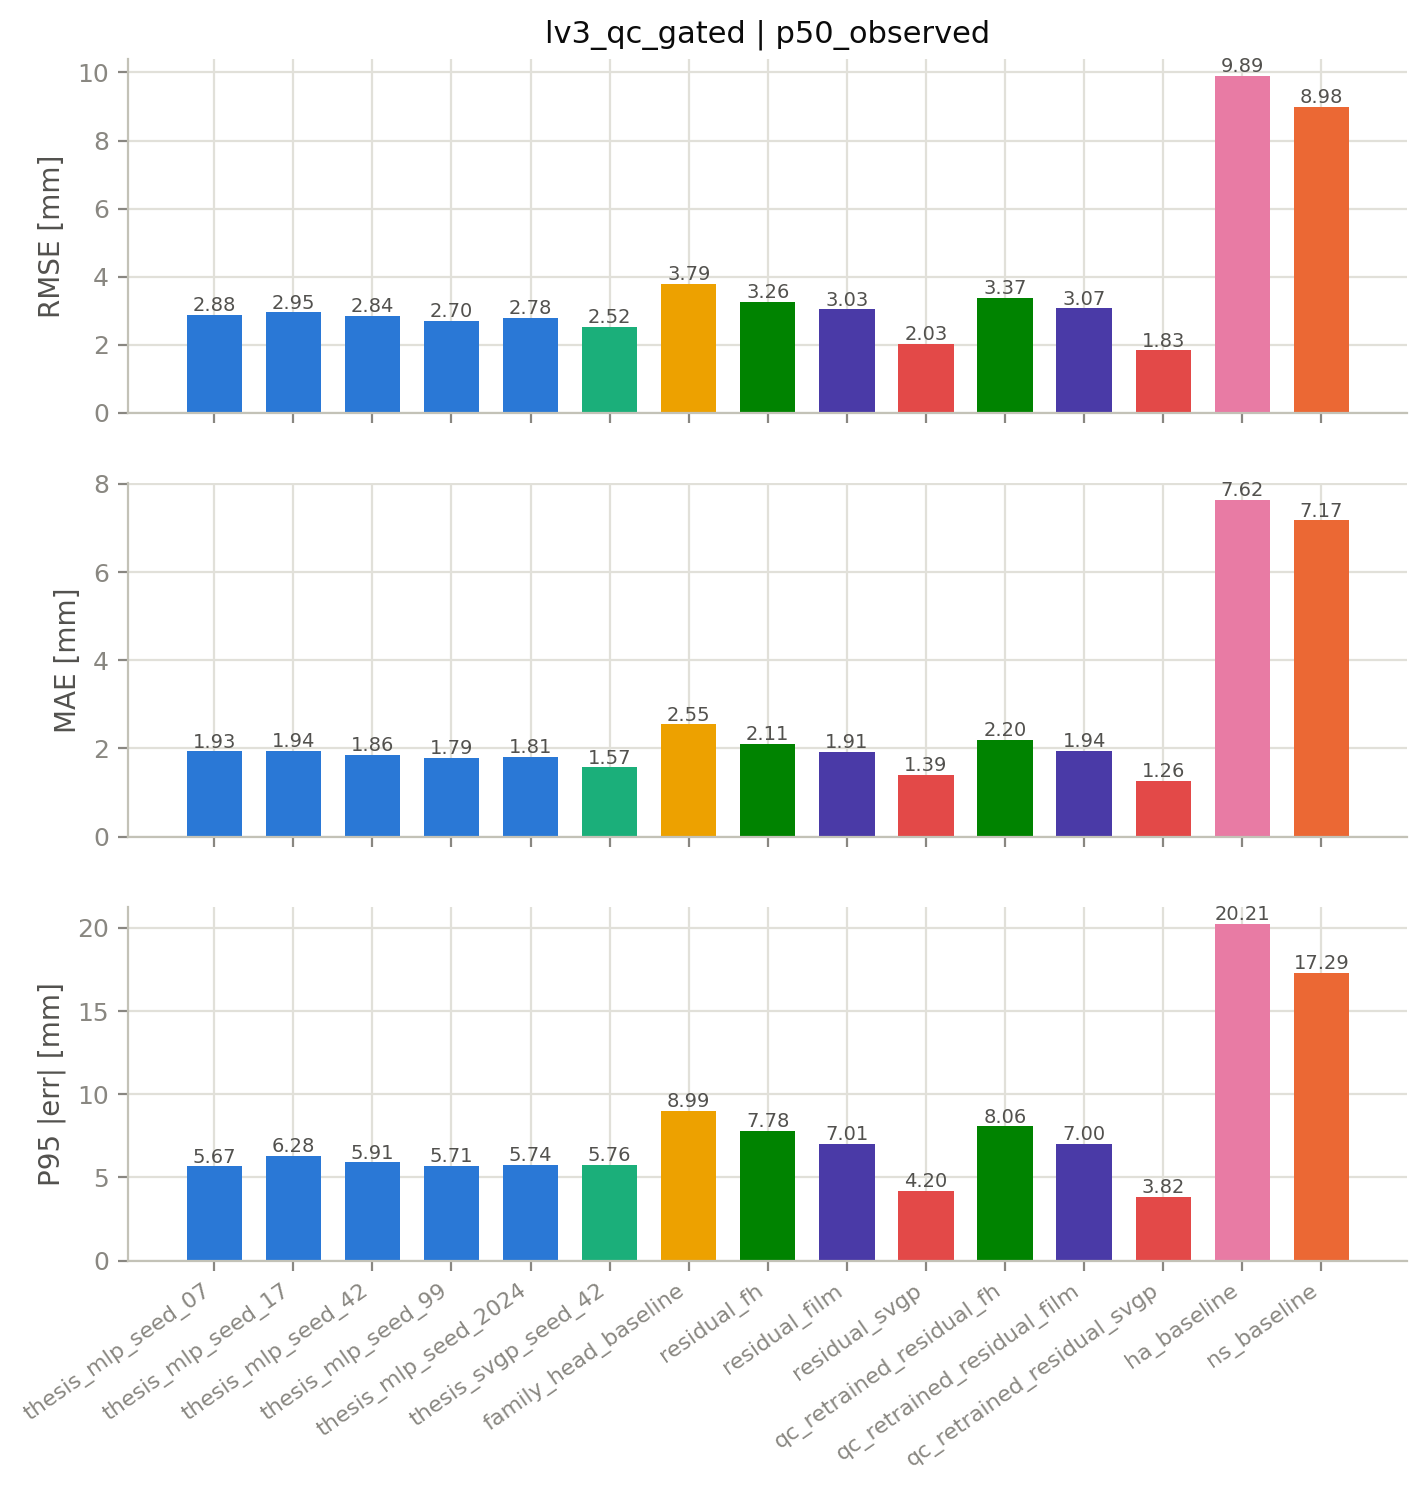
\includegraphics[width=\linewidth]{images/eval_20260709/metric_bars_rmse_mae_p95_p50_observed.png}
\caption{Observed P50 protocol.}
\end{subfigure}
\hfill
\begin{subfigure}[t]{0.49\linewidth}
\centering
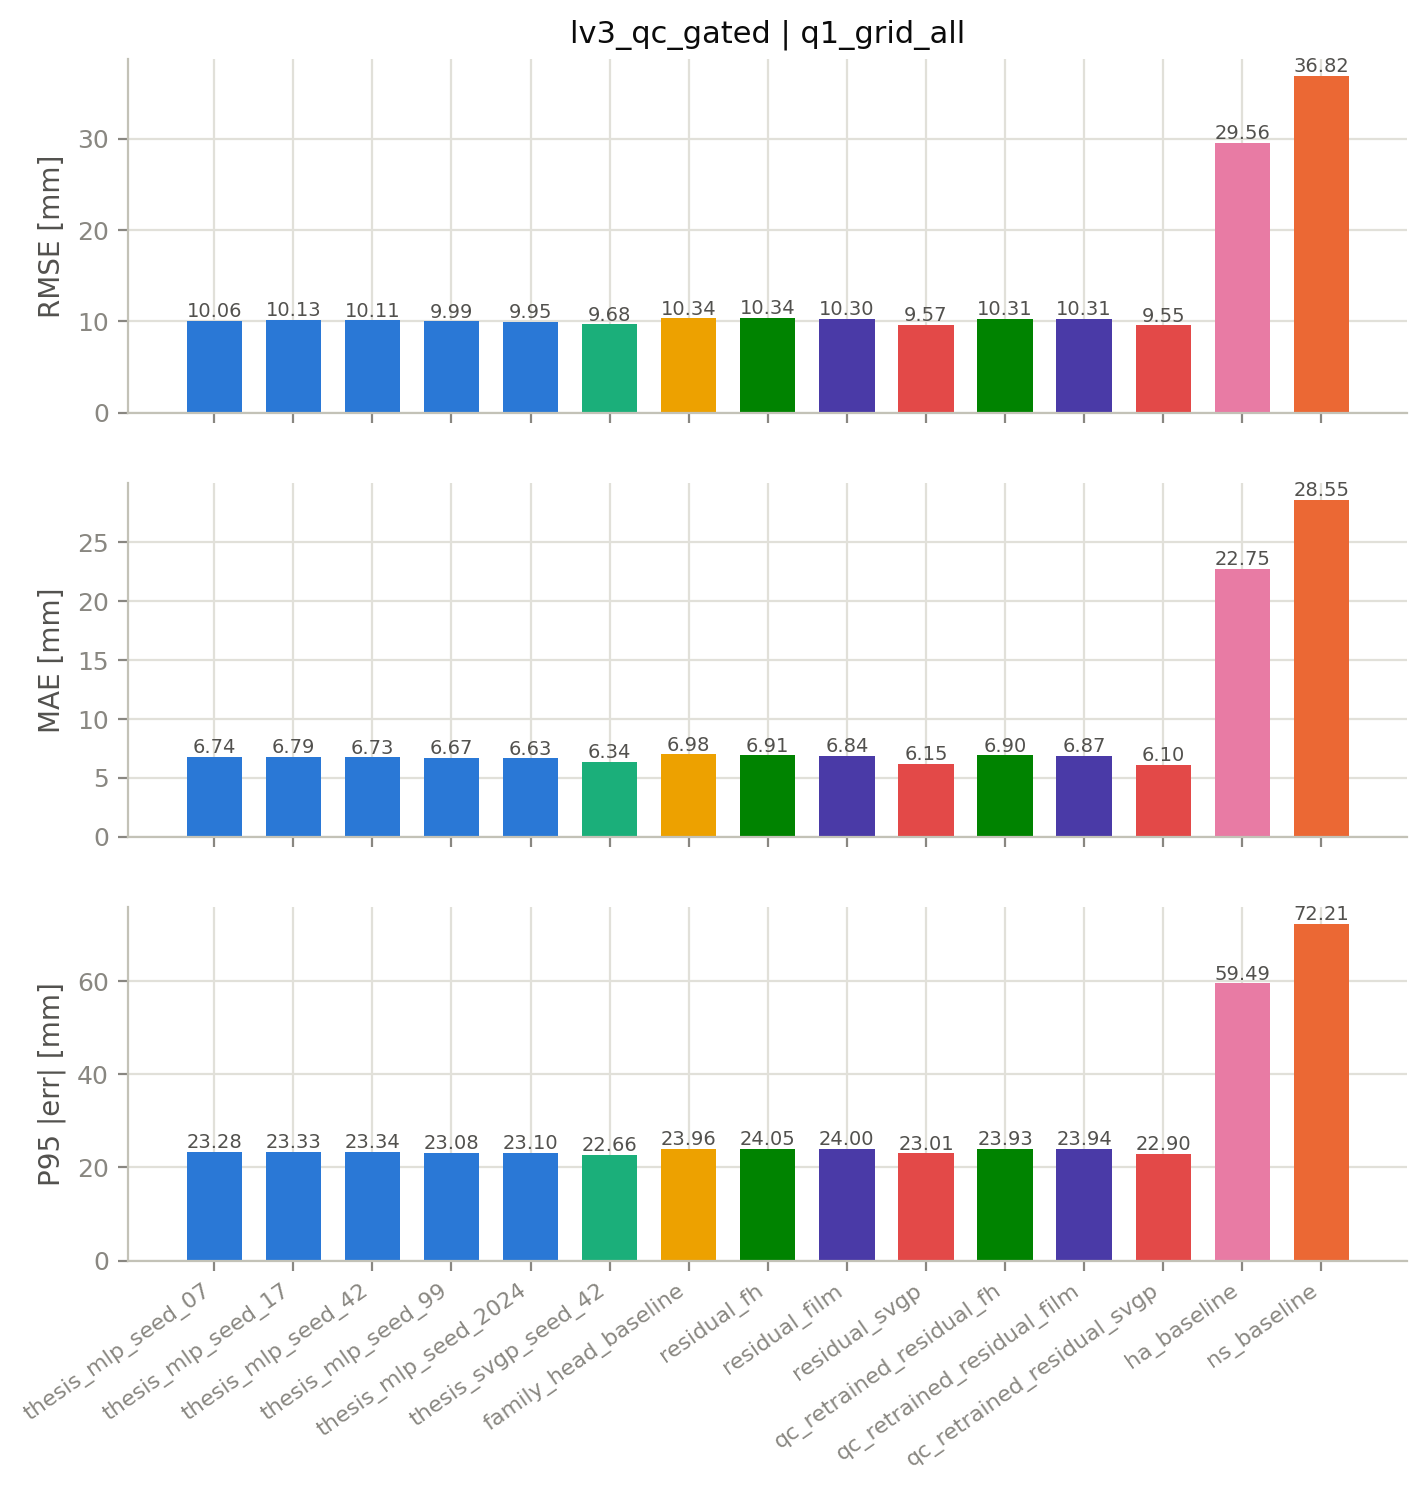
\includegraphics[width=\linewidth]{images/eval_20260709/metric_bars_rmse_mae_p95_q1_grid_all.png}
\caption{q1 continuation grid.}
\end{subfigure}
\caption{Secondary protocol point-error comparisons. The P50 protocol isolates representative behavior inside the measurement window, whereas the q1 grid tests continuation behavior from the fitted reduced-order target.}
\label{fig:secondary-protocol-bars-rewrite}
\end{figure}

\subsubsection{Censoring-Inclusive Full-Clean Check}
\label{sec:full-clean-supplement}

The full-clean CDF protocol is the censoring-inclusive counterpart of the
primary table: it evaluates the same held-out population without excluding
right-censored regions. In the refreshed bundle this protocol is regenerated on
the same QC-gated root as the primary verdict, so the two tables differ only in
whether right-censored regions are included. It remains a supplementary check
rather than the headline verdict because the primary comparison deliberately
excludes regions where the target itself is shaped by field-of-view censoring.

On the QC-gated root the refreshed full-clean table contains 689{,}162 held-out
CDF prediction points, of which 148{,}795 (21.6\%) lie in right-censored
regions. In the earlier archived bundle the same censoring pressure was
quantified at the trajectory level: 9{,}630 of 24{,}316 cleaned held-out
trajectories (39.6\%) were right-censored, which is the spatial censoring ratio
quoted in the data chapters. Both views make the same point: treating the last
visible point as a physical terminal penetration would be a material protocol
error rather than a bookkeeping detail. On the refreshed censoring-inclusive
view, the five-seed production MLP reaches \SI{4.584}{mm} RMSE, \SI{3.211}{mm}
MAE, \SI{+0.829}{mm} bias, and conservative \(1\sigma/2\sigma\) coverage of
0.869/0.986. The Stage~3 SVGP is again the stronger point predictor (RMSE
\SI{4.440}{mm} with 95\% interval [4.373, 4.499], MAE \SI{3.109}{mm}) but with
sharper, less conservative coverage (0.706/0.942), and both physical baselines
remain far behind (\SI{11.187}{mm} and \SI{10.442}{mm} RMSE, corresponding to
MLP reductions of 59.0\% and 56.1\%). The censoring-inclusive ordering is
therefore the same as the primary uncensored verdict.

\begin{table}[t]
\centering
\footnotesize
\setlength{\tabcolsep}{3pt}
\begin{tabular}{@{}L{0.28\linewidth}rrrrrr@{}}
\toprule
Model & RMSE & MAE & Bias & P95 & 1$\sigma$ & 2$\sigma$ \\
\midrule
Calibrated Hiroyasu--Arai & 11.187 & 8.605 & +0.193 & 22.765 & 0.618 & 0.914 \\
Naber--Siebers with delay term & 10.442 & 8.117 & -0.545 & 21.089 & 0.640 & 0.921 \\
Three-stage MLP, selected anchor-off screening surrogate, 5-seed mean & 4.584 & 3.211 & +0.829 & 9.036 & 0.869 & 0.986 \\
SVGP, Stage~3 mode & \textbf{4.440} & \textbf{3.109} & -0.145 & \textbf{9.028} & 0.706 & 0.942 \\
\bottomrule
\end{tabular}
\caption{Refreshed supplementary censoring-inclusive comparison on the QC-gated full-clean CDF set (689{,}162 points), which includes right-censored regions. Error units are mm; P95 is the 95th-percentile absolute error. The MLP row is the five-seed mean and the SVGP row is the Stage~3 seed-42 reference; cluster-bootstrap 95\% confidence intervals for RMSE, MAE, and bias are exported with the run artifacts. The diagnostic KD variant reported in the archived 2026-05-21 version of this table is not part of the refreshed roster and is omitted here.}
\label{tab:external-clean-headline}
\end{table}

\begin{figure}[t]
\centering
\begin{subfigure}[t]{0.49\linewidth}
\centering
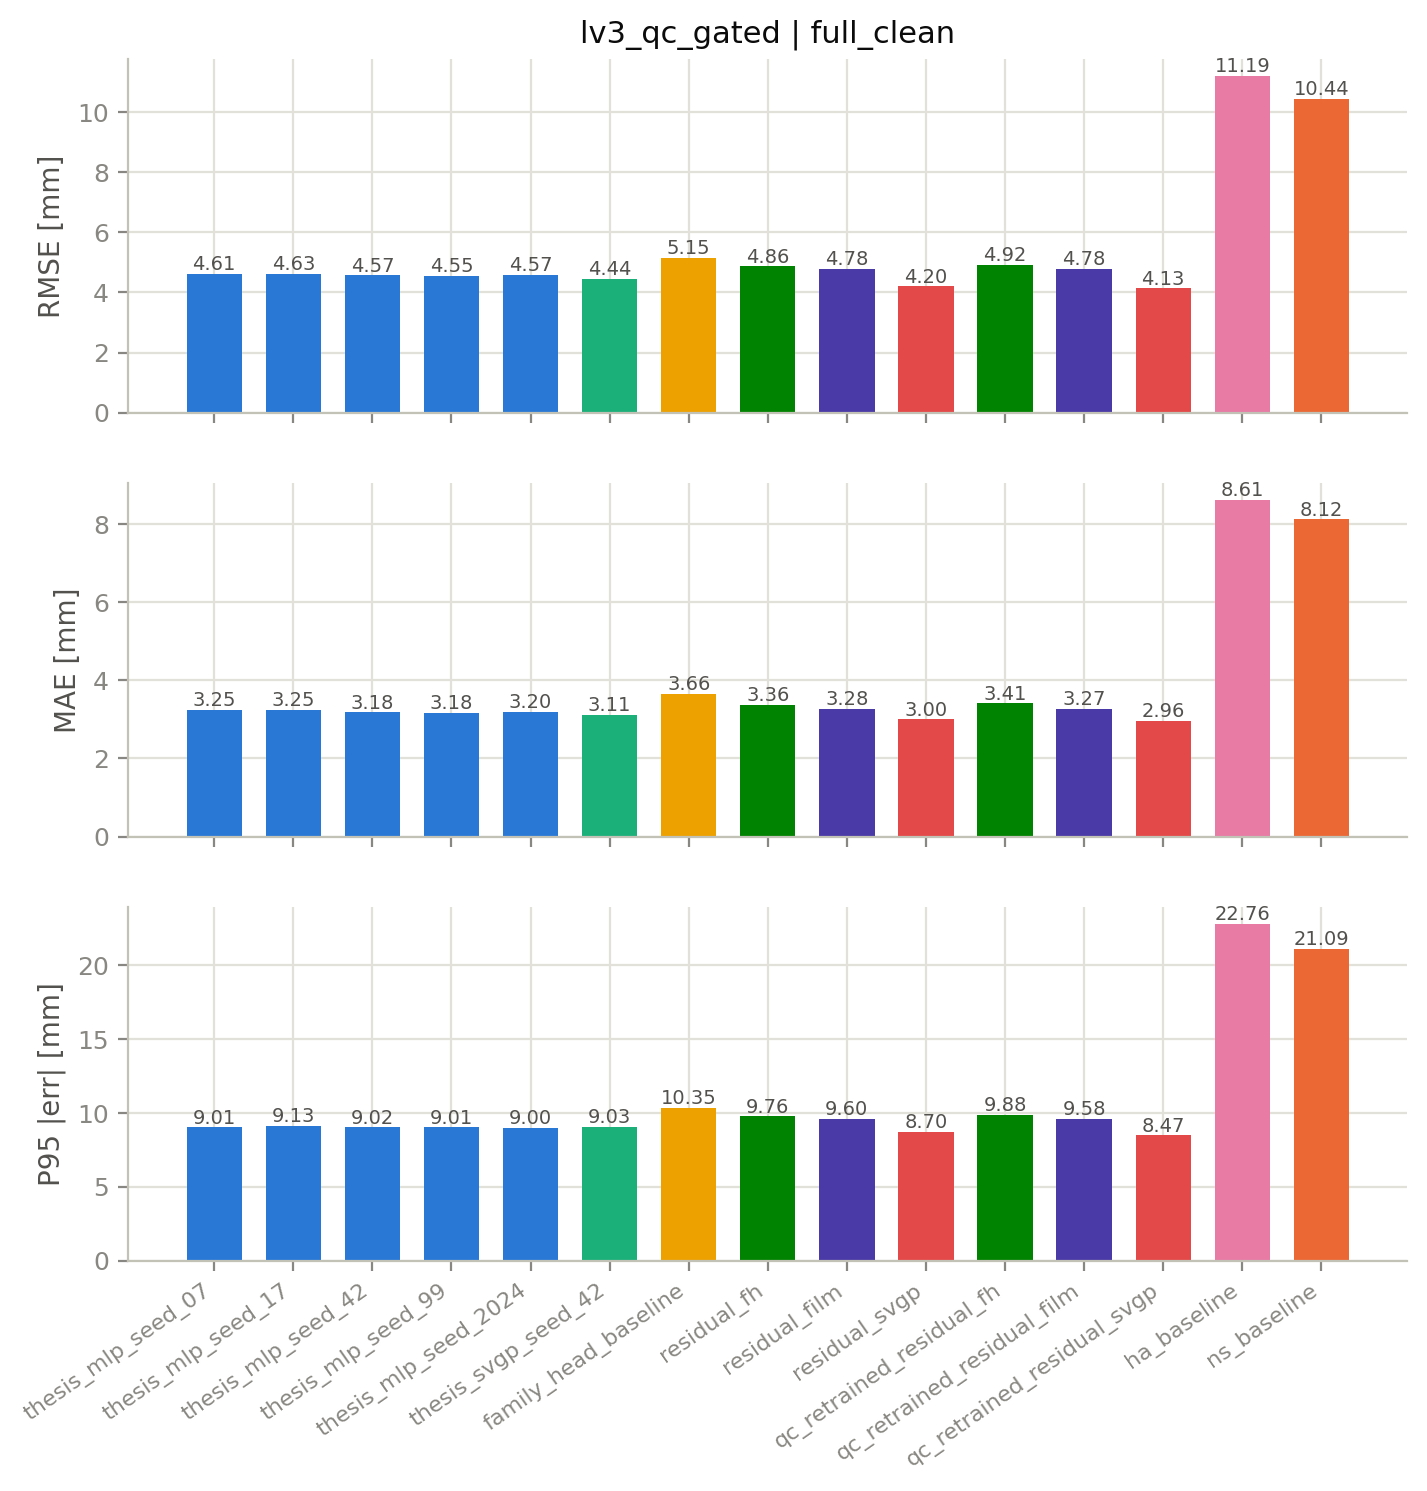
\includegraphics[width=\linewidth]{images/eval_20260709/metric_bars_rmse_mae_p95_full_clean.png}
\caption{Point and tail errors.}
\end{subfigure}
\hfill
\begin{subfigure}[t]{0.49\linewidth}
\centering
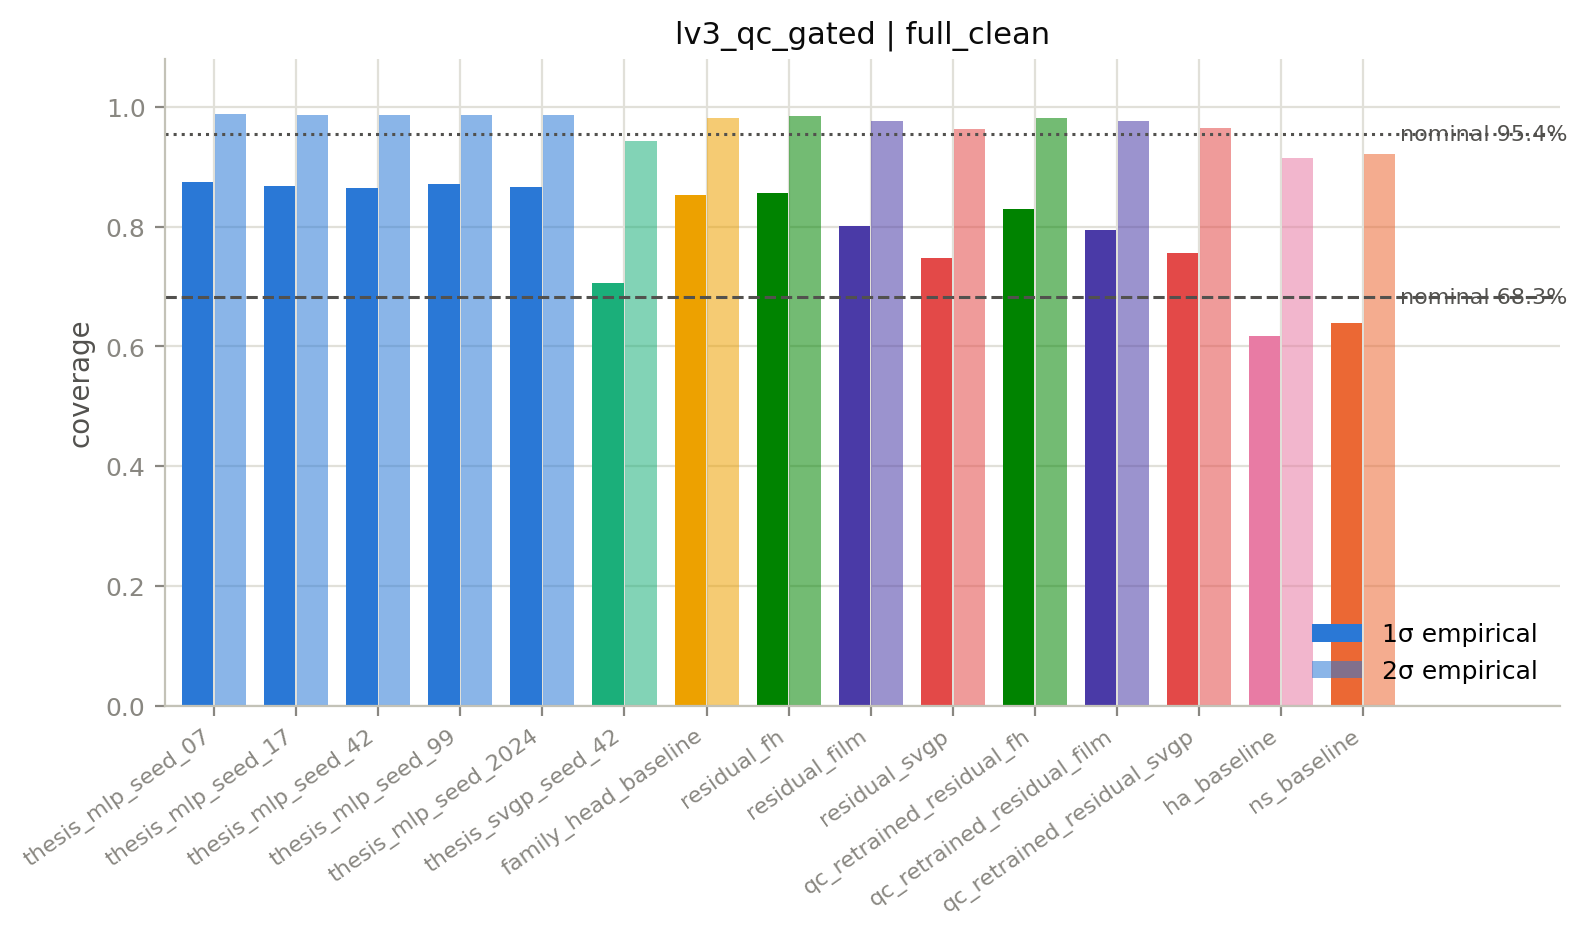
\includegraphics[width=\linewidth]{images/eval_20260709/coverage_comparison_full_clean.png}
\caption{Empirical coverage.}
\end{subfigure}
\caption{Refreshed full-clean CDF supplementary diagnostics on the QC-gated root. The censoring-inclusive comparison reproduces the primary accuracy--coverage trade-off; the primary thesis verdict remains the QC-gated uncensored CDF protocol.}
\label{fig:full-clean-diagnostics}
\end{figure}

\begin{figure}[t]
\centering
\begin{subfigure}[t]{0.49\linewidth}
\centering
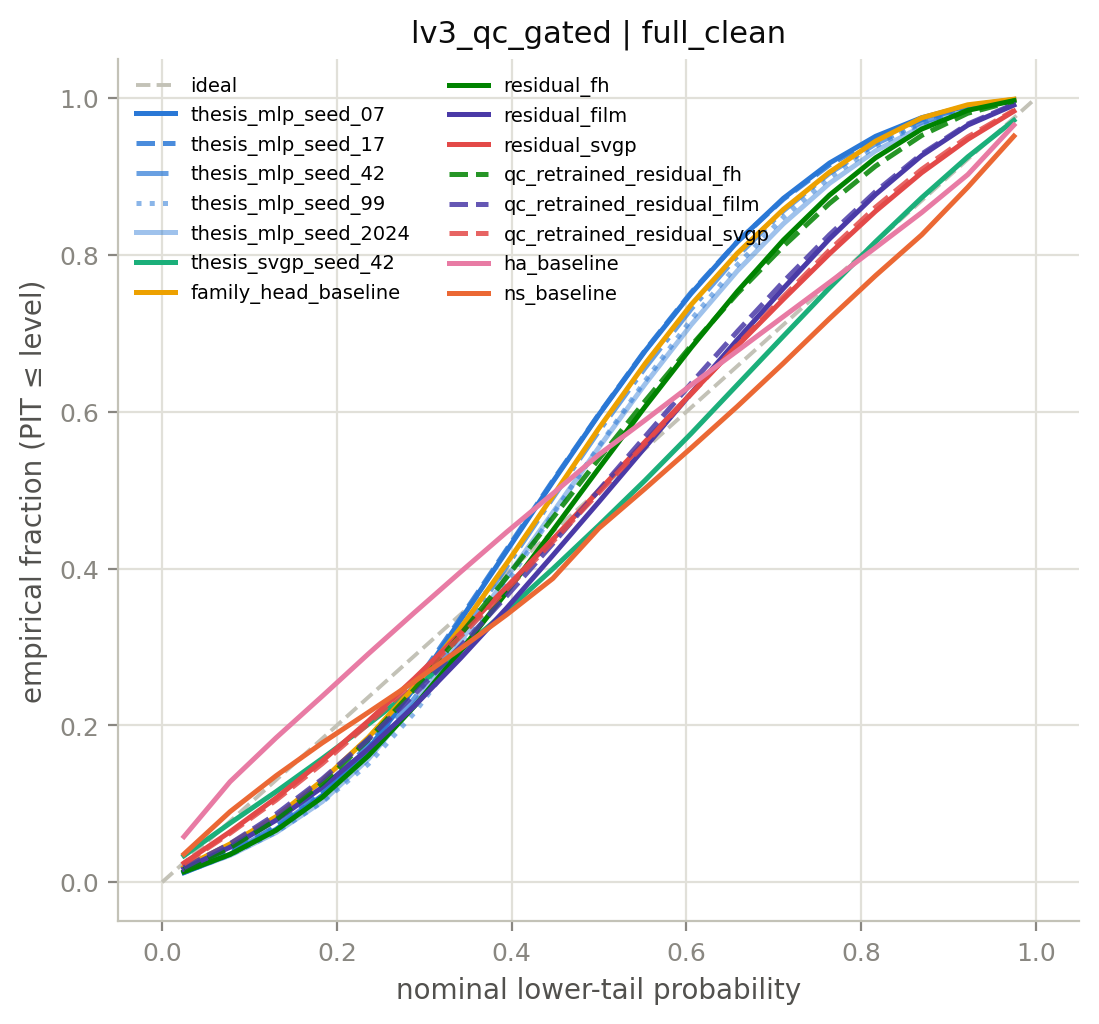
\includegraphics[width=\linewidth]{images/eval_20260709/reliability_overlay_full_clean.png}
\caption{Reliability diagram.}
\end{subfigure}
\hfill
\begin{subfigure}[t]{0.49\linewidth}
\centering
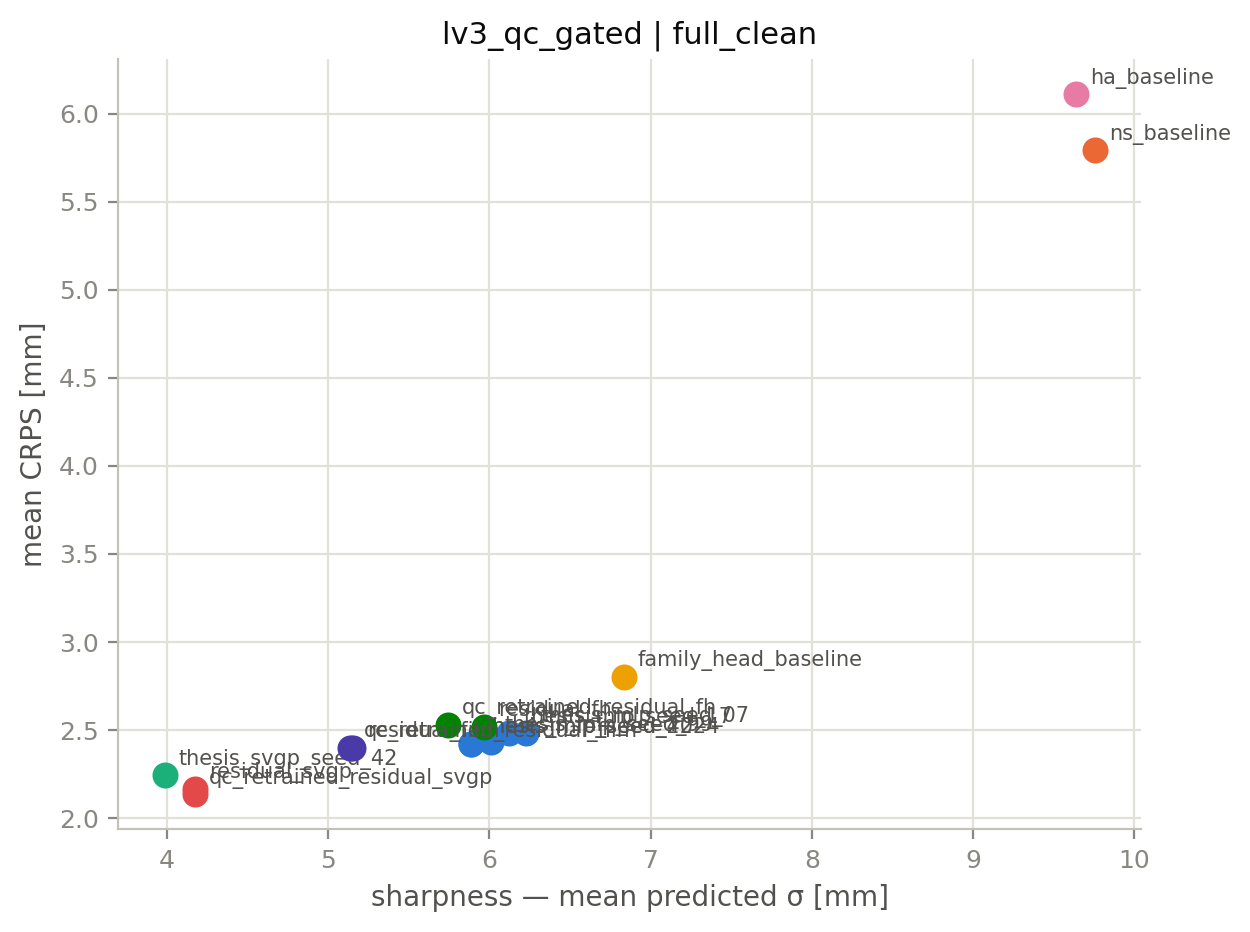
\includegraphics[width=\linewidth]{images/eval_20260709/crps_sharpness_scatter_full_clean.png}
\caption{CRPS--sharpness plane.}
\end{subfigure}
\caption{Refreshed full-clean probabilistic calibration diagnostics. The SVGP is sharper with lower CRPS, while the production MLP has wider and more conservative intervals; the censoring-inclusive view supports the same accuracy--coverage trade-off as the primary protocol.}
\label{fig:full-clean-calibration}
\end{figure}

\FloatBarrier

\subsection{Calibration and Distributional Behavior}
\label{sec:calibration-distributional}

Coverage at a few sigma levels is only a coarse summary, so the refreshed
pipeline also exports reliability curves, PIT histograms, CRPS, NLL, interval
scores, and sigma-bin calibration tables for the probabilistic fixed-table
sets. These diagnostics reinforce the same trade-off. The production MLP is
conservative: its mean predicted standard deviation is about
\SI{5.96}{mm}, and its \(1\sigma\) coverage is about 0.888. The mainline
single-output SVGP is sharper, with mean predicted standard deviation about
\SI{3.73}{mm}, lower CRPS (\SI{2.063}{mm}), and lower RMSE, but less
conservative \(1\sigma\) coverage. The post-hoc QC-retrained residual-SVGP
pushes CRPS lower again (\SI{1.988}{mm}) while still remaining less
conservative than the production MLP.

This distinction matters for the downstream screening interface. A model with
the best mean prediction is not automatically the safest rank-oriented
screening surrogate if its uncertainty intervals are too narrow for edge
conditions. Conversely, conservative MLP intervals should not be oversold as a
certified false-negative guarantee. They are evidence of a deliberately cautious
predictive distribution under the measured protocol.

\begin{figure}[t]
\centering
\begin{subfigure}[t]{0.49\linewidth}
\centering

\includegraphics[width=\linewidth]{images/eval_20260709/reliability_overlay.png}
\caption{Reliability overlay.}
\end{subfigure}
\hfill
\begin{subfigure}[t]{0.49\linewidth}
\centering

\includegraphics[width=\linewidth]{images/eval_20260709/crps_sharpness_scatter.png}
\caption{CRPS--sharpness plane.}
\end{subfigure}
\caption{Distributional diagnostics on the primary QC-gated uncensored CDF table. The SVGP variants occupy the sharper and lower-CRPS region, while the production MLP trades point sharpness for conservative coverage.}
\label{fig:distributional-diagnostics-rewrite}
\end{figure}

\begin{figure}[t]
\centering
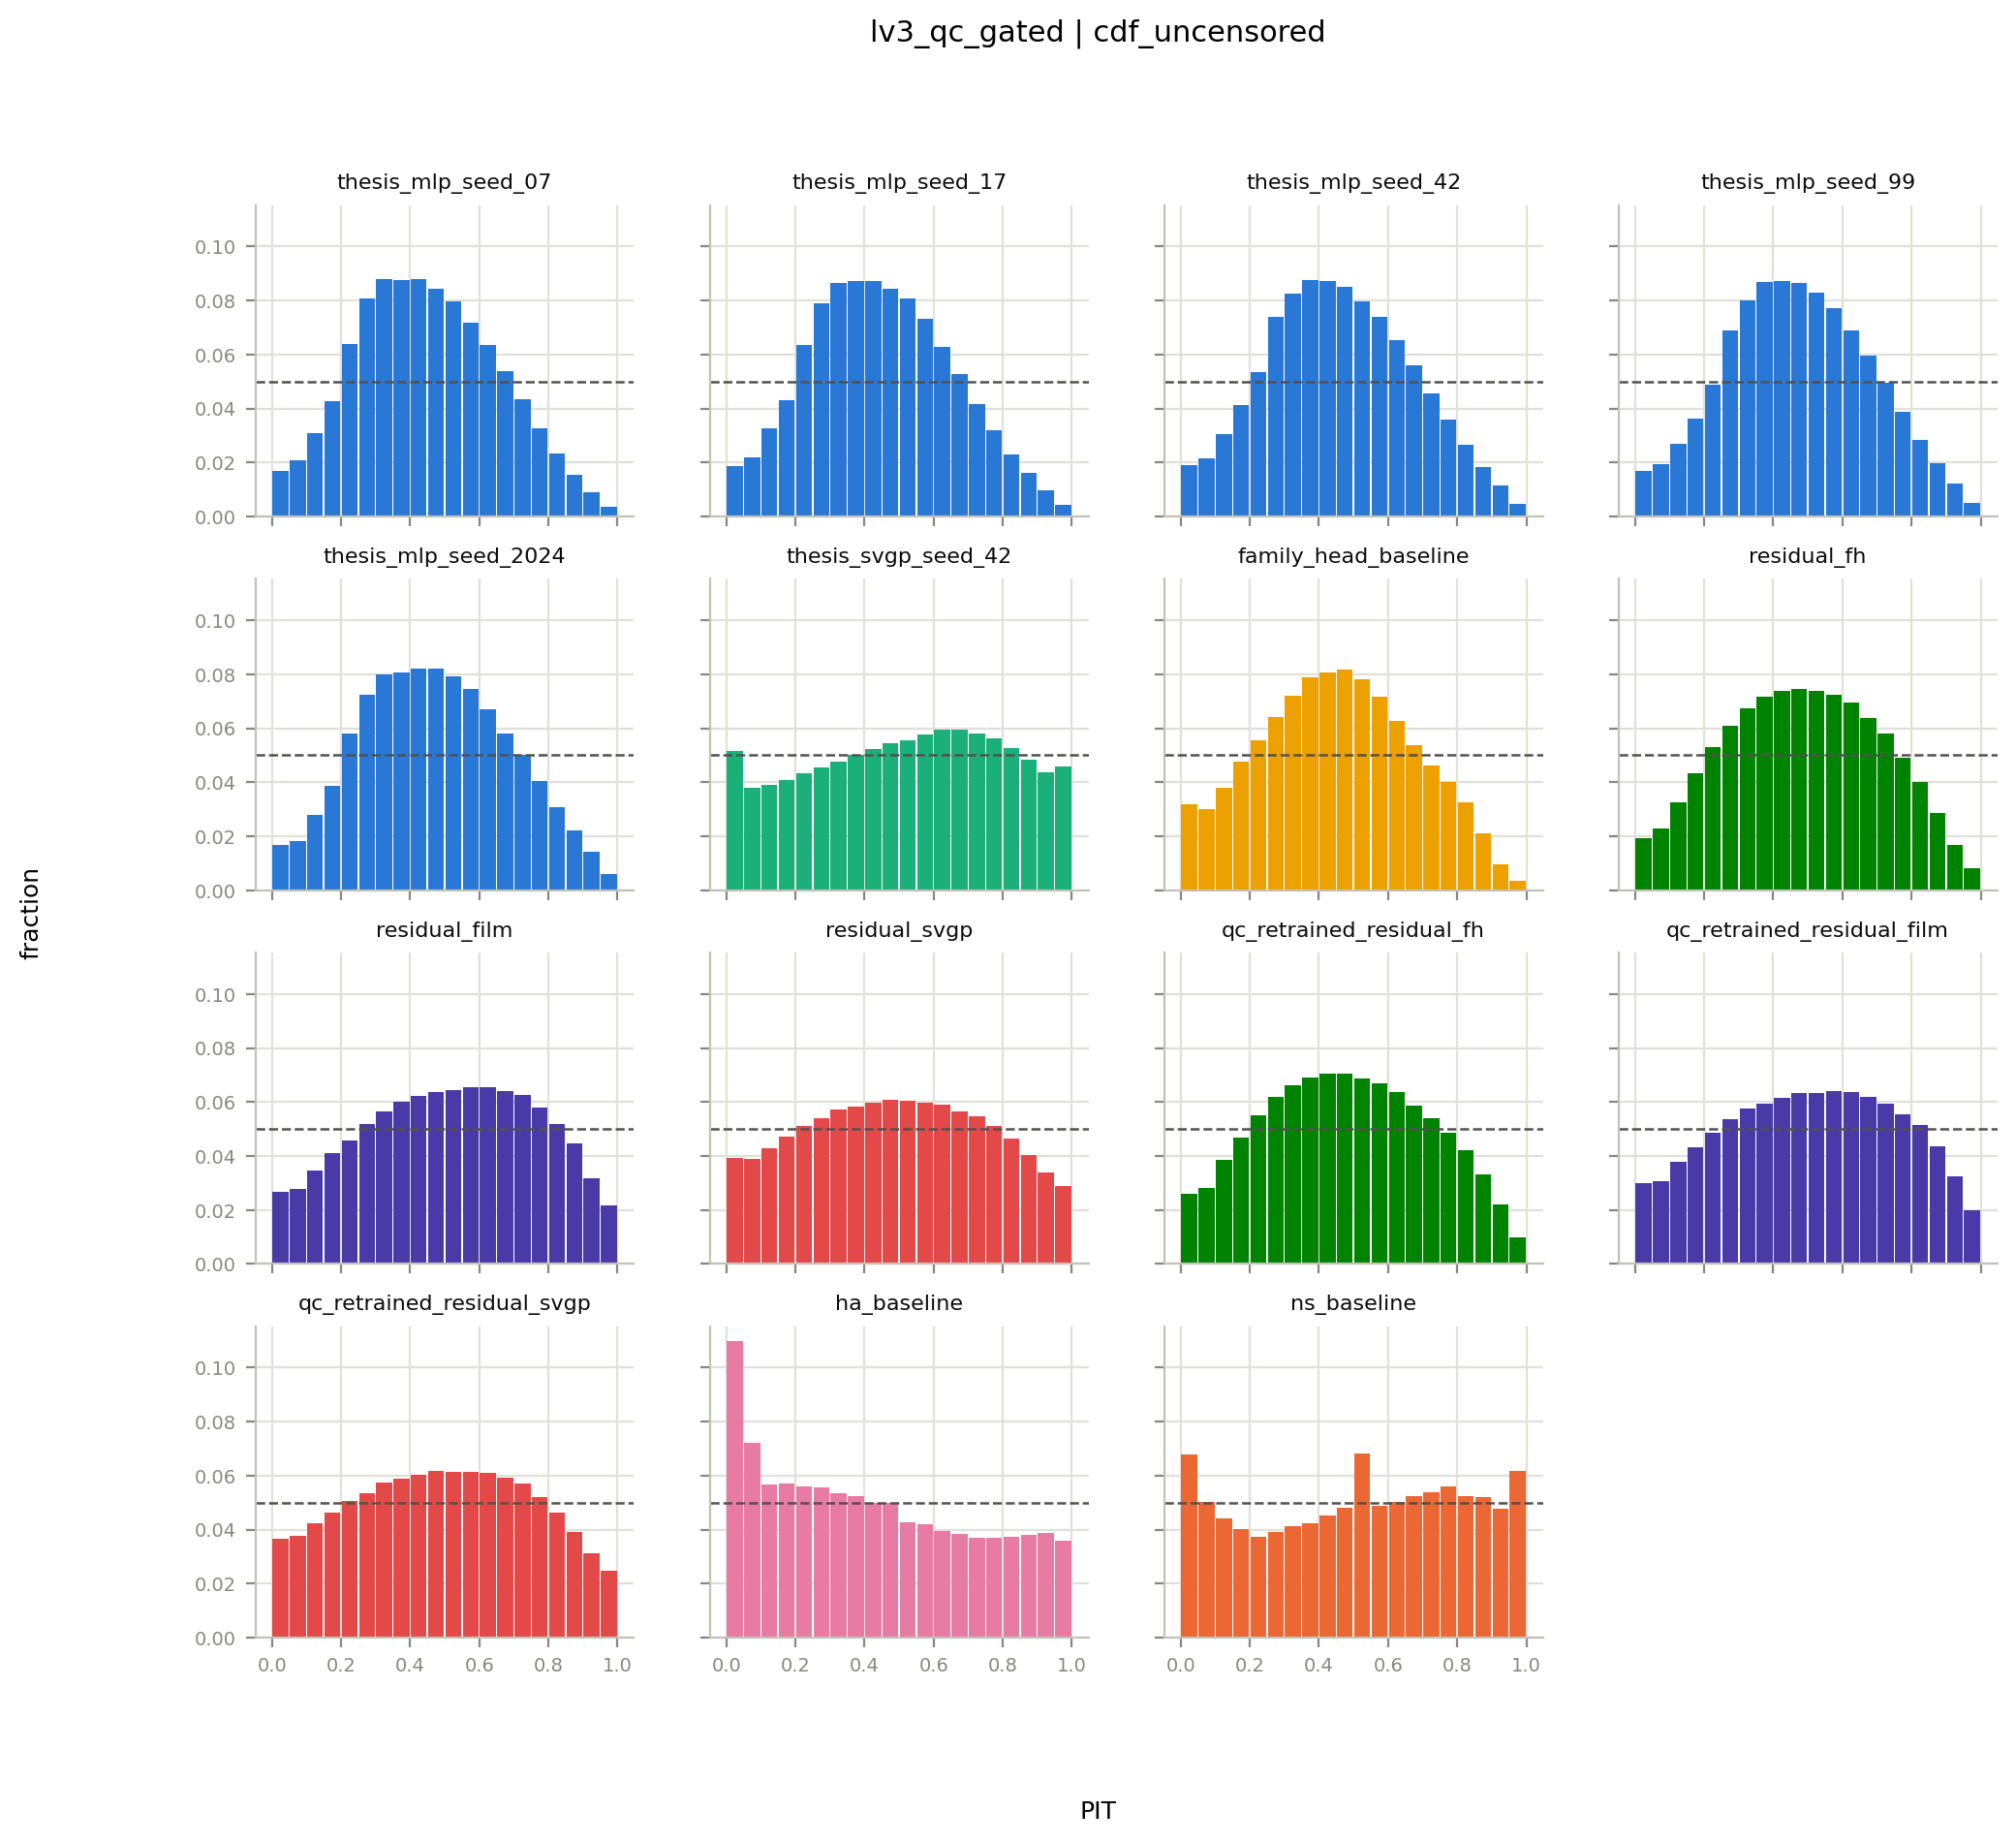
\includegraphics[width=0.86\linewidth]{images/eval_20260709/pit_histograms_grid.png}
\caption{PIT histograms for the refreshed primary comparison. These histograms complement the reliability overlay by exposing model-wise deviations from a uniform predictive distribution.}
\label{fig:pit-grid-rewrite}
\end{figure}

\FloatBarrier

\subsection{Cross-Nozzle Transfer and Failure Boundaries}
\label{sec:lono-boundaries-rewrite}
\label{sec:lono-transfer-en}
\label{sec:lono-transfer-zh}
\label{sec:svgp-lono-comparison-en}
\label{sec:svgp-lono-comparison-zh}

The fixed-table results above test in-domain performance on held-out points
from the cleaned dataset root. They do not answer whether the surrogate can
generalize to an entirely unseen injector. That question is handled by the
Leave-One-Nozzle-Out protocol retained from the archived thesis artifacts.

Under the five-fold LONO protocol holding out Nozzle0, Nozzle1, Nozzle2,
Nozzle4, and Nozzle5 in turn, the Stage~3 SVGP achieves a lower average RMSE
than the MLP: \(\SI{10.16}{mm}\pm\SI{9.57}{mm}\) versus
\(\SI{12.55}{mm}\pm\SI{12.46}{mm}\). Excluding the out-of-design-family
Nozzle0 fold, the comparison remains in the same direction:
\(\SI{5.95}{mm}\pm\SI{1.98}{mm}\) for the SVGP and
\(\SI{7.00}{mm}\pm\SI{1.18}{mm}\) for the MLP. The coverage story is more
intertwined: after removing Nozzle0, the \(1\sigma\) coverage is nearly equal
(0.697 for SVGP and 0.696 for MLP), while the MLP has higher \(2\sigma\)
coverage (0.923 versus 0.890). The \(\pm\) terms in this paragraph are
cross-fold standard deviations from the archived single-seed LONO run, not
multi-seed training uncertainty.

The main transfer verdict is therefore sharper than the in-domain verdict. The
SVGP is the better point-transfer backbone under LONO. The MLP is retained not
because it wins every transfer metric, but because it is conservative
in-domain, exposes the auxiliary onset output used by the screening GUI, and
supports cheap ablation of the training curriculum.

\begin{figure}[t]
\centering
\begin{subfigure}[t]{0.49\linewidth}
\centering
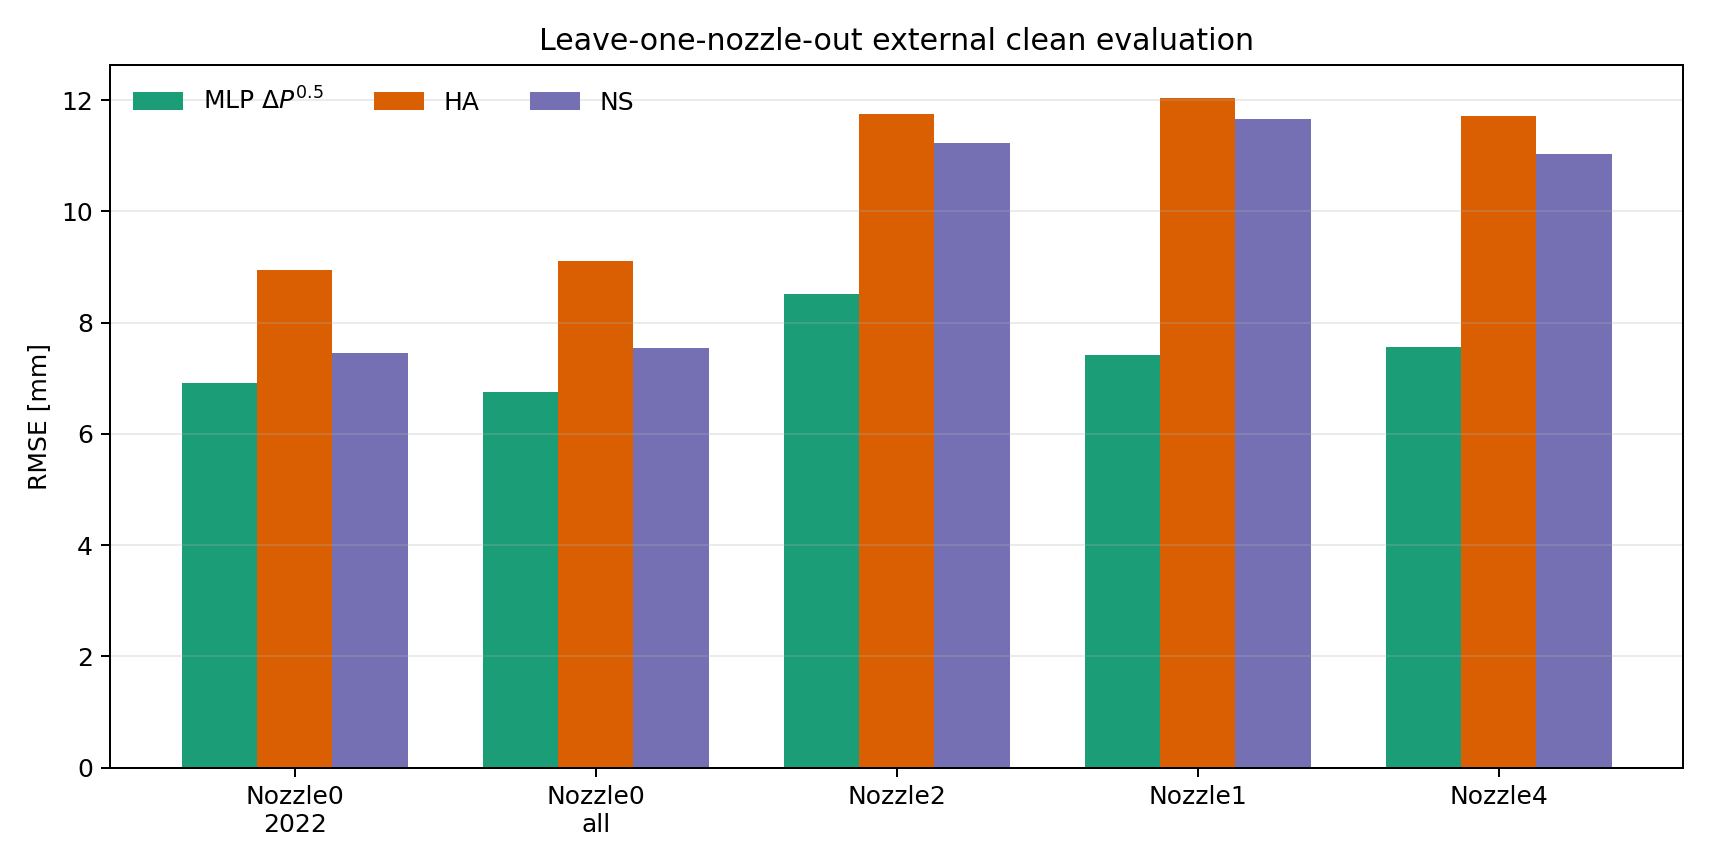
\includegraphics[width=\linewidth]{images/lono_20260509/lono_rmse_by_fold.png}
\caption{Per-fold RMSE.}
\end{subfigure}
\hfill
\begin{subfigure}[t]{0.49\linewidth}
\centering
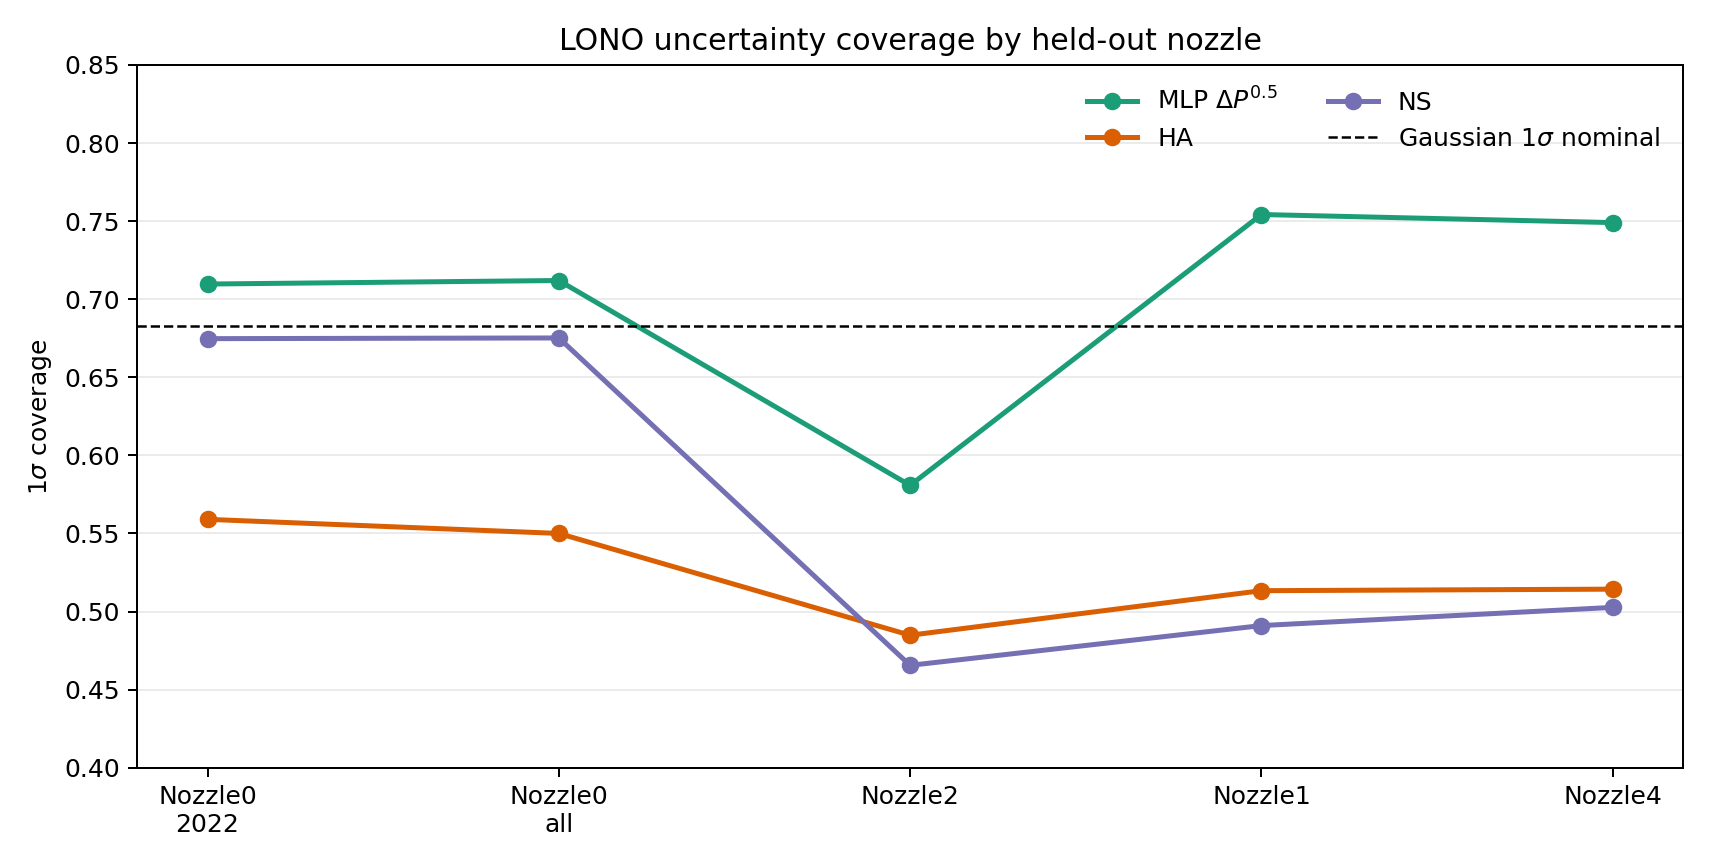
\includegraphics[width=\linewidth]{images/lono_20260509/lono_coverage_by_fold.png}
\caption{Per-fold \(1\sigma\) coverage.}
\end{subfigure}
\caption{Archived LONO diagnostics for the Stage~3 MLP and SVGP. Nozzle0 dominates the high standard deviation and marks the out-of-design-family boundary for both architectures.}
\label{fig:lono-boundary-rewrite}
\label{fig:svgp-lono-comparison}
\label{fig:svgp-lono-comparison-zh}
\end{figure}

The Nozzle0 collapse should not be hidden by averaging. Nozzle0 is the only
factory-fresh reference injector in the campaign and has an early-time
penetration envelope that the modified-injector training population does not
represent. It is better interpreted as a cross-design-family extrapolation
failure than as an ordinary fold. This boundary is scientifically useful: it
states where the learned surrogate requires either additional family coverage,
trunk-level adaptation, or retraining.

\subsubsection{Physical Failure-Mode Check: Nozzle 3}
\label{sec:nozzle3-failure-rewrite}

The LONO averages identify transfer boundaries, but they do not show the raw
spray morphology behind difficult cases. An archived Nozzle~3 condition
provides a useful failure anatomy by pairing Phantom high-speed Mie images with
the corresponding plume-by-plume penetration curves
(Figure~\ref{fig:failure-mode-nozzle3-rewrite}). In the early window from
\SI{0.6}{ms} to about \SI{1.0}{ms}, several bottom-right plumes remain short
and discontinuous while other holes have already formed continuous jets. The
penetration curves show the same event as a flat-top or step-like trajectory:
a small leading liquid mass appears first, decelerates, and is later overtaken
by a faster main jet.

This image evidence is consistent with wake-driven catch-up or transient
orifice-throttling interpretations, but it is not a causal diagnosis. The
experiment does not contain simultaneous gas velocity, internal-flow
visualization, or liquid-mass identity tracking. The direct modeling conclusion
is narrower and more useful: a smooth monotone continuation target cannot
represent abrupt step-like curvature changes without distorting the target or
the predictive uncertainty. These cases explain why some within-family
conditions remain difficult even after the global LONO and fixed-table metrics
look acceptable.

\begin{figure}[p]
\centering
\begin{minipage}{0.24\linewidth}
\centering
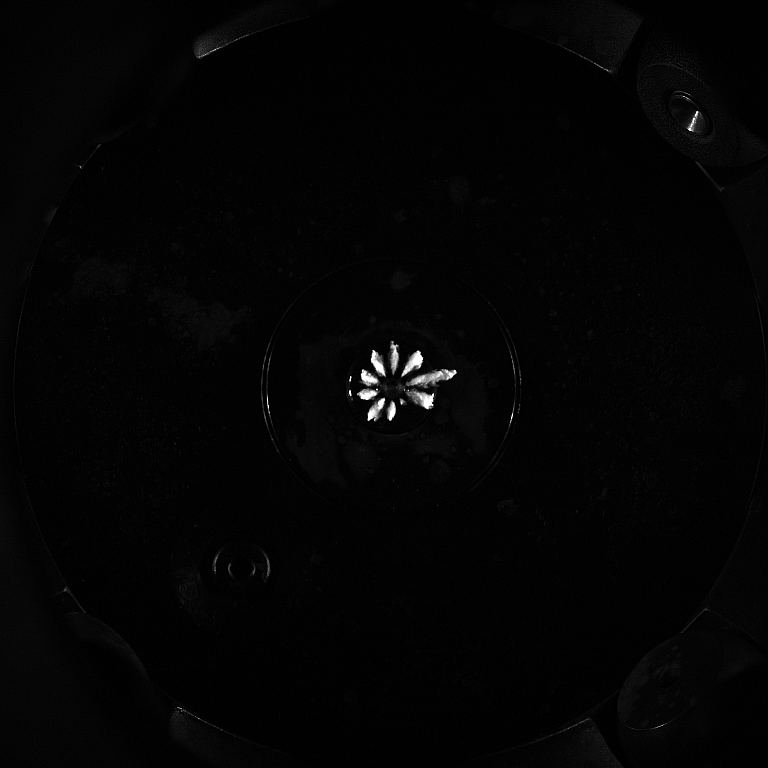
\includegraphics[width=\linewidth]{images/failure_mode_nozzle3/phantom_t3.png}\\
{\footnotesize (a) \(t\approx\SI{0.6}{ms}\)--\(\SI{0.8}{ms}\)}
\end{minipage}
\hfill
\begin{minipage}{0.24\linewidth}
\centering
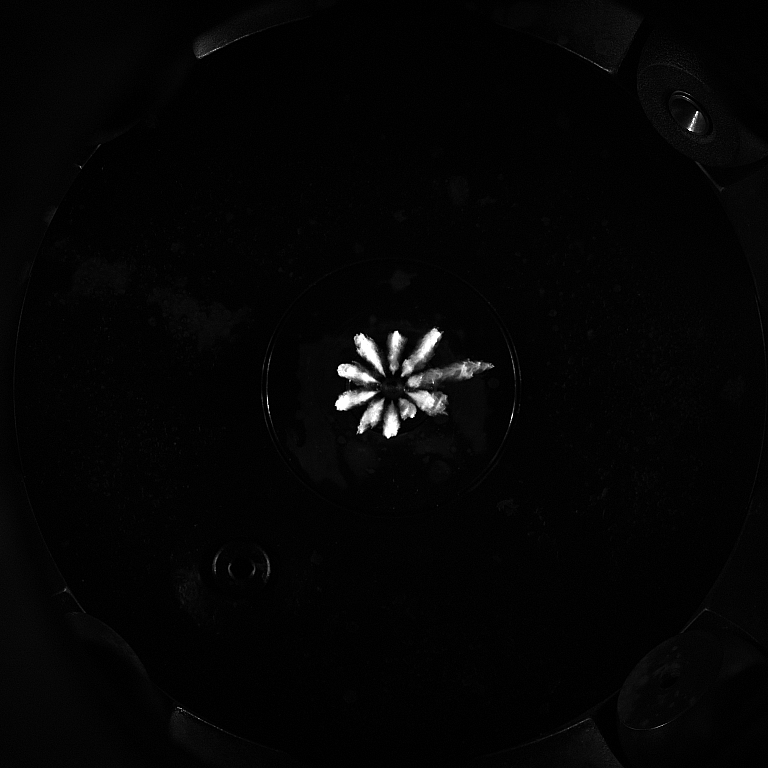
\includegraphics[width=\linewidth]{images/failure_mode_nozzle3/phantom_t4.png}\\
{\footnotesize (b) \(t\approx\SI{0.8}{ms}\)}
\end{minipage}
\hfill
\begin{minipage}{0.24\linewidth}
\centering
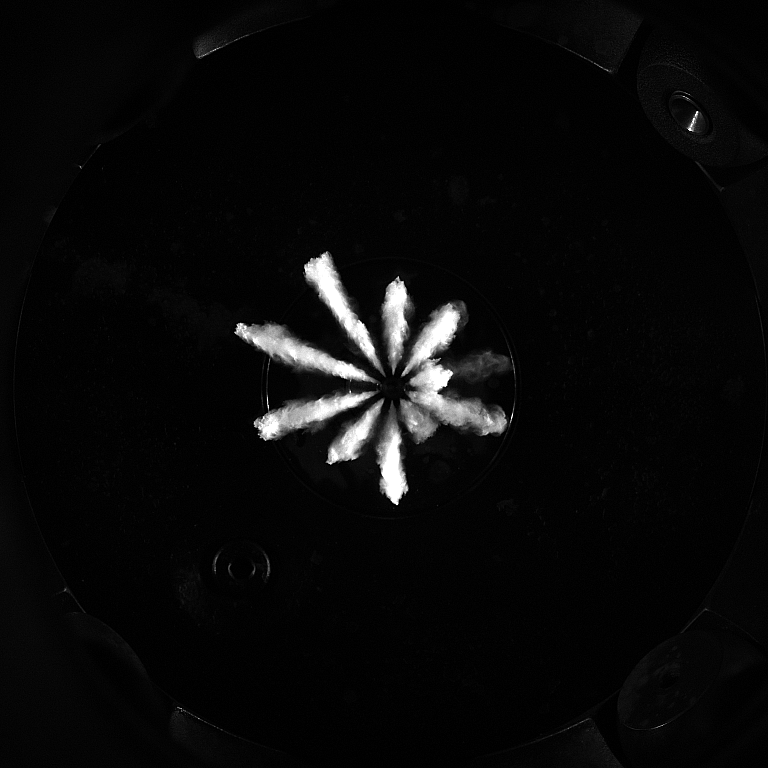
\includegraphics[width=\linewidth]{images/failure_mode_nozzle3/phantom_t5.png}\\
{\footnotesize (c) \(t\approx\SI{1.0}{ms}\)}
\end{minipage}
\hfill
\begin{minipage}{0.24\linewidth}
\centering
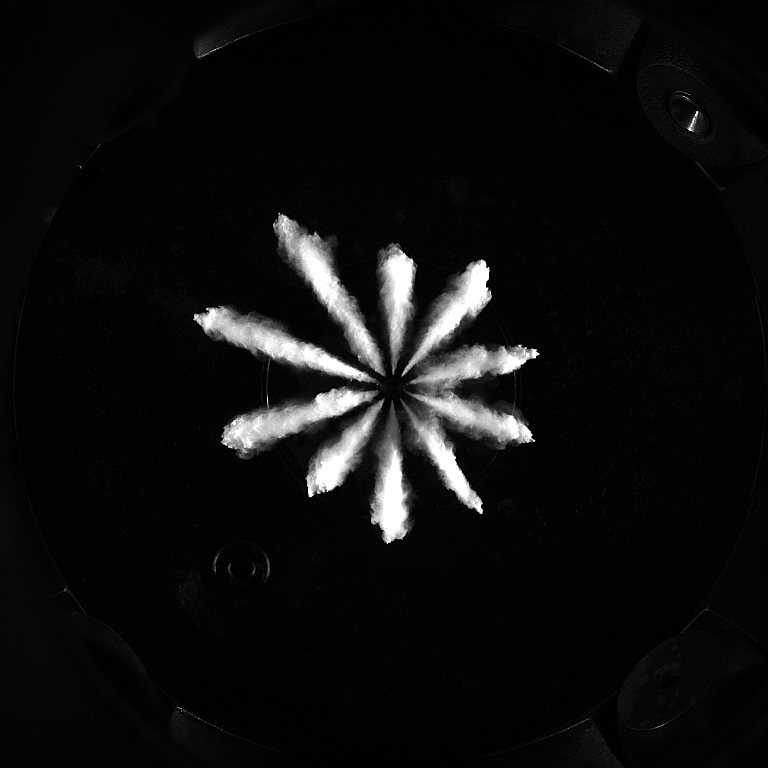
\includegraphics[width=\linewidth]{images/failure_mode_nozzle3/phantom_t6.png}\\
{\footnotesize (d) \(t>\SI{1.0}{ms}\)}
\end{minipage}

\vspace{1em}
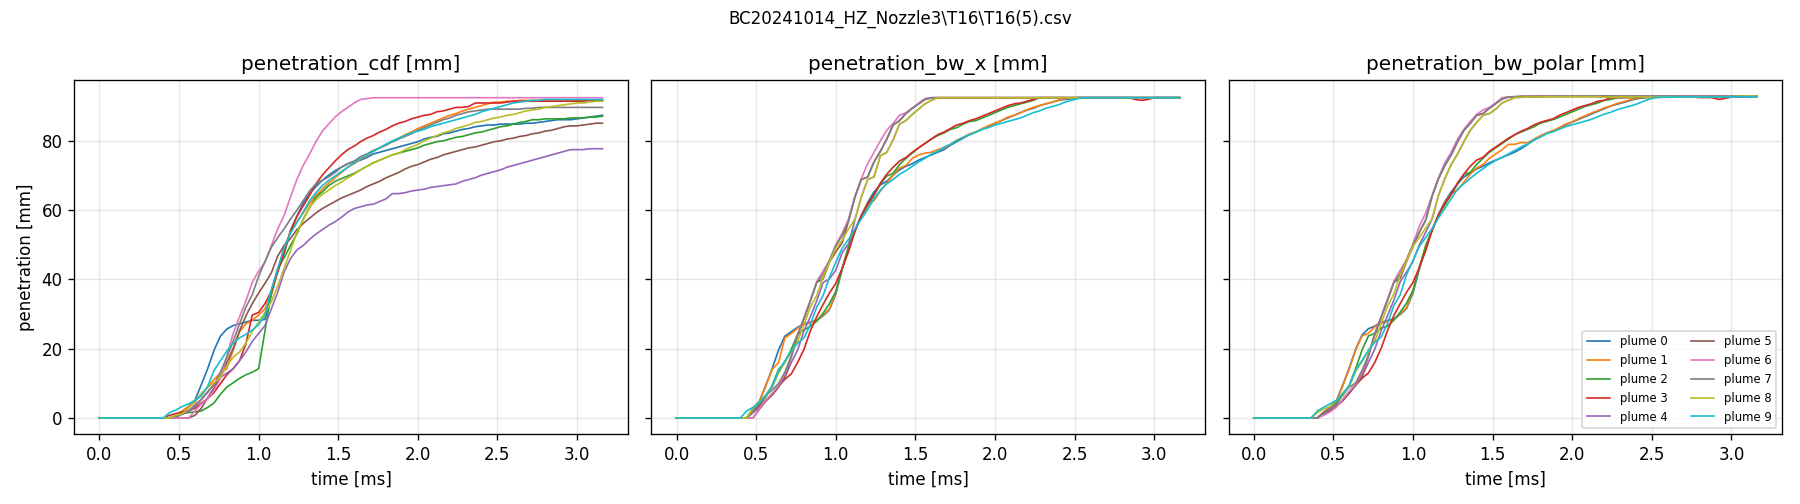
\includegraphics[width=0.95\linewidth]{images/failure_mode_nozzle3/nozzle3_t16_plot.png}
\caption{Visual evidence and corresponding penetration curves for an extreme transient spray in Nozzle~3. The image sequence shows initially short, discontinuous bottom-right plumes followed by a later main jet, while the lower curves show the associated flat-top and step-like penetration behavior. The figure supports a modeling failure-mode interpretation, not a uniquely identified fluid-mechanical cause.}
\label{fig:failure-mode-nozzle3-rewrite}
\label{fig:failure-mode-nozzle3}
\label{fig:failure-mode-nozzle3-zh}
\end{figure}

\FloatBarrier

\subsection{Why the MLP Workflow Was Retained}
\label{sec:why-mlp-retained-rewrite}
\label{sec:mlp-ablation-affordability-en}
\label{sec:mlp-ablation-affordability-zh}

The preceding sections make the model trade-off explicit. The SVGP family is
stronger for point prediction and LONO transfer. The MLP workflow is retained
for a different reason: it makes the staged curriculum, uncertainty behavior,
onset auxiliary output, and screening deployment auditable within a Master's
thesis compute budget. The ablation evidence explains that choice.

\subsubsection{Curriculum Ablations}
\label{sec:curriculum-ablations-rewrite}
\label{sec:stage2-anchor-ablation-en}
\label{sec:stage2-anchor-ablation-zh}

The Stage~2 anchor ablation tested whether an early-time mean anchor and an
early-time sigma anchor improve the teacher used by Stage~3. The
\(\mu\)-anchor-only variant is the most defensible teacher setting: it lowers
the five-fold LONO RMSE from \SI{14.54}{mm} to \SI{12.73}{mm}, improves MAE,
and avoids the overconfident behavior introduced by the double
\(\mu+\sigma\) anchor. The improvement is concentrated in a difficult fold,
which is precisely where a physically motivated anchor should matter; the full
archived tables, including the per-fold breakdown and the bias and coverage
columns, are collected in Appendix~\ref{app:evaluation-diagnostics}.

The Stage~3 supervision-mix ablation then tests how raw observations and
teacher guidance should be blended. The uncertain-regime mixed variant obtains
the lowest average LONO RMSE and MAE, but the margin between Stage~3 variants
is only about \SI{0.21}{mm}, far below the cross-fold standard deviation. This
should be read as a mild selection preference, not as a sweeping architectural
claim.

\begin{table}[t]
\centering
\scriptsize
\setlength{\tabcolsep}{4pt}
\begin{tabularx}{\linewidth}{@{}L{0.29\linewidth}rrY@{}}
\toprule
Ablation result & RMSE & MAE & Main interpretation \\
\midrule
Stage~2 no anchor & 14.54 & 10.80 & Leaves early-time slack that can collapse on difficult folds. \\
Stage~2 \(\mu\)-anchor only & \textbf{12.73} & \textbf{9.86} & Best teacher setting; improves bias and 2-sigma coverage. \\
Stage~2 \(\mu+\sigma\) anchor & 13.05 & 10.06 & Over-tightens early uncertainty without compensating accuracy gain. \\
\addlinespace
Stage~3 baseline regime & 12.68 & 9.97 & Competitive but not best. \\
Stage~3 uncertain-regime mixed & \textbf{12.55} & \textbf{9.80} & Best LONO point score, with small margins relative to fold variance. \\
Stage~3 anchor-off & 12.73 & 9.86 & Highest archived 2-sigma LONO coverage among these variants. \\
\bottomrule
\end{tabularx}
\caption{Condensed curriculum ablation verdict. The numbers are archived LONO means. The purpose of this table is not to create another leaderboard, but to show which design decisions are actually supported by the ablation evidence.}
\label{tab:curriculum-ablation-condensed}
\end{table}

\begin{figure}[t]
\centering
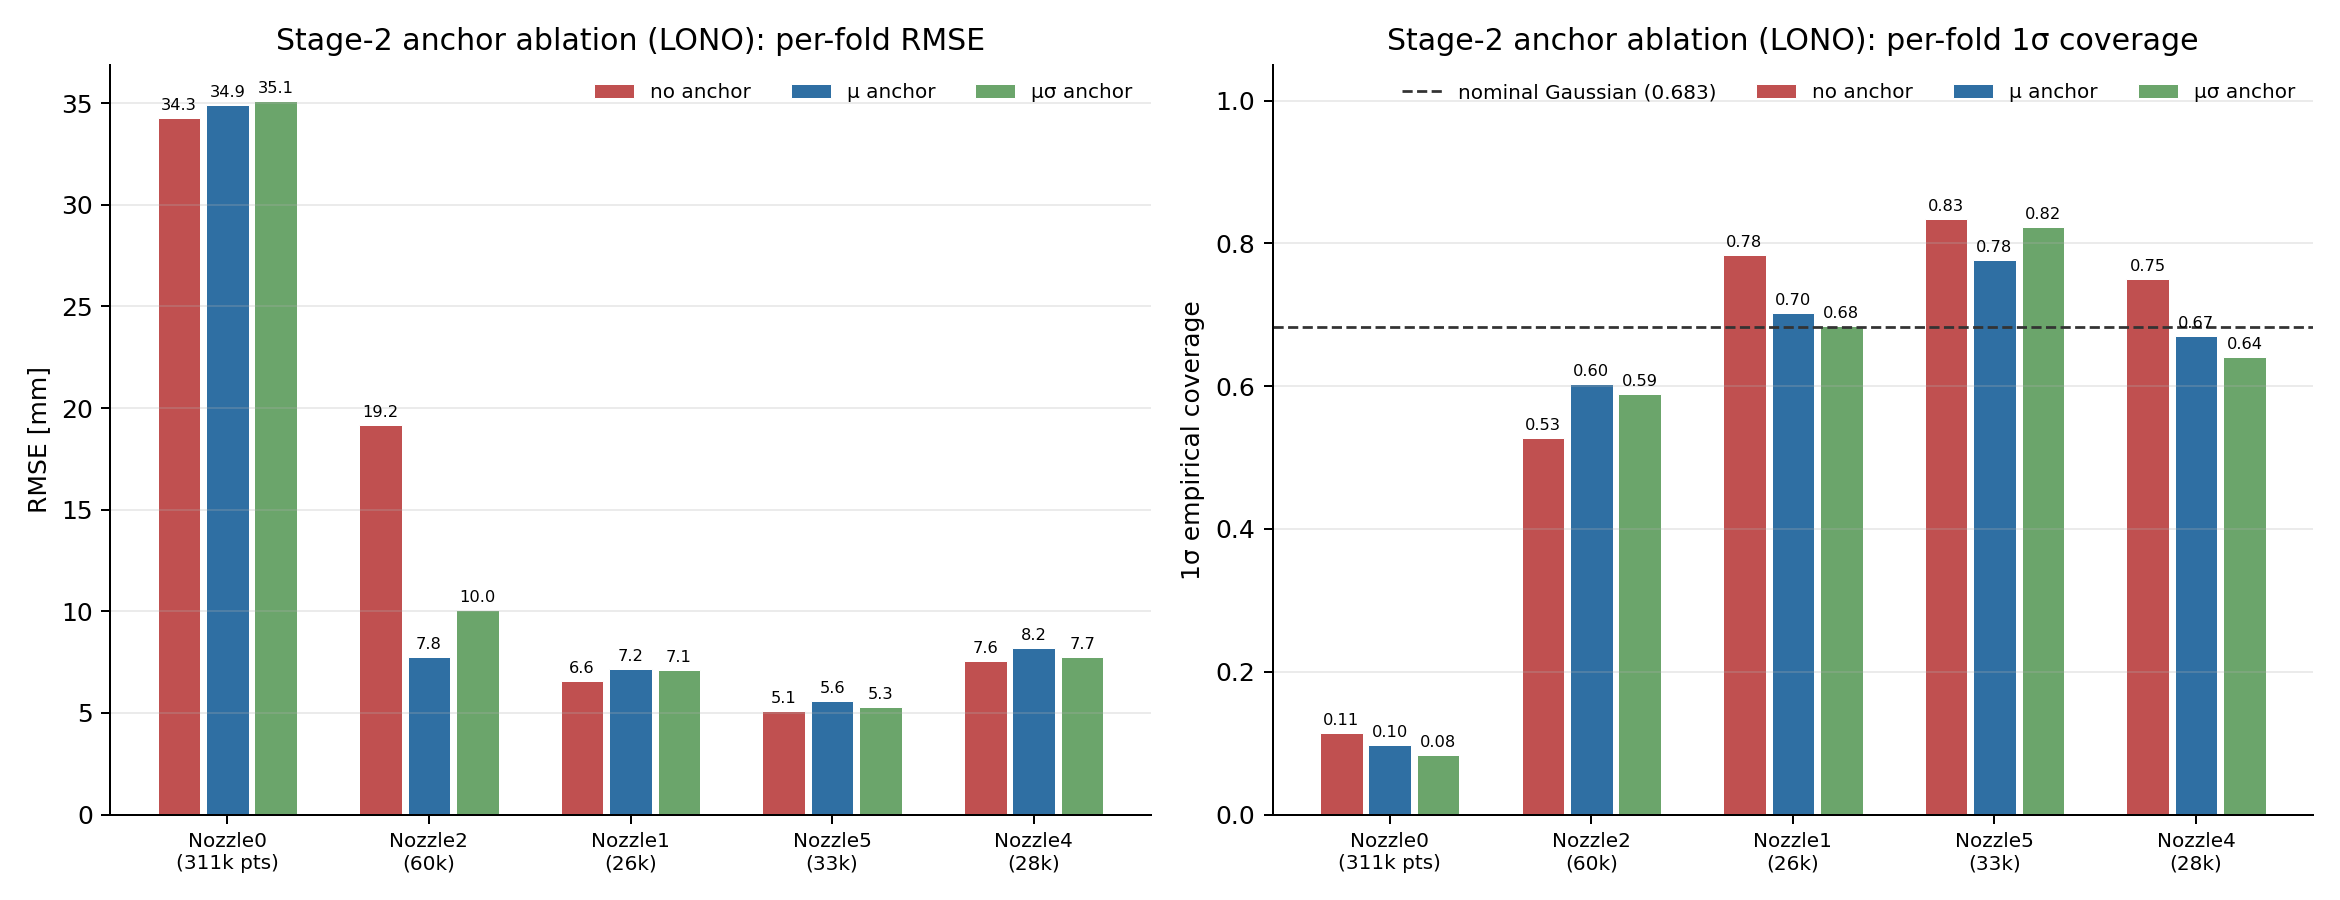
\includegraphics[width=0.92\linewidth]{images/stage2_anchor_ablation.png}
\caption{Archived Stage~2 anchor ablation. The \(\mu\)-anchor-only teacher is retained because it improves the difficult transfer cases without forcing early uncertainty to become overconfident.}
\label{fig:stage2-ablation-rewrite}
\end{figure}

\subsubsection{KD Loss Formulation and Near-Cap Bias}
\label{sec:kd-loss-rewrite}
\label{sec:kd-form-fix-en}
\label{sec:kd-form-fix-zh}

A separate Stage~3 diagnostic exposed a systematic under-prediction near the
field-of-view cap. The Stage~2 teacher was nearly unbiased near this cap, but
the earlier forward-KL student introduced approximately \(-\SI{2.70}{mm}\) of
additional near-cap bias. Replacing the KL term with a mixed mean-MSE plus
log-variance-MSE distillation loss removes the variance-inflation escape route:
the selected \(\lambda_\sigma=5.0\) setting pulls the near-cap bias back to
about \(-\SI{0.57}{mm}\), close to the teacher's \(-\SI{0.59}{mm}\). Across
five seeds, the aggregate near-cap RMSE is about \(\SI{4.881}{mm}\) with a
seed standard deviation of \SI{0.024}{mm}, and the near-cap bias standard
deviation is \SI{0.079}{mm}. The archived slice-level evidence---the loss
formulation, the supervision-regime and censoring-slice table, and the
calibration-drift diagnostics---is preserved in
Appendix~\ref{app:evaluation-diagnostics}.

\begin{figure}[t]
\centering
\begin{subfigure}[t]{0.49\linewidth}
\centering
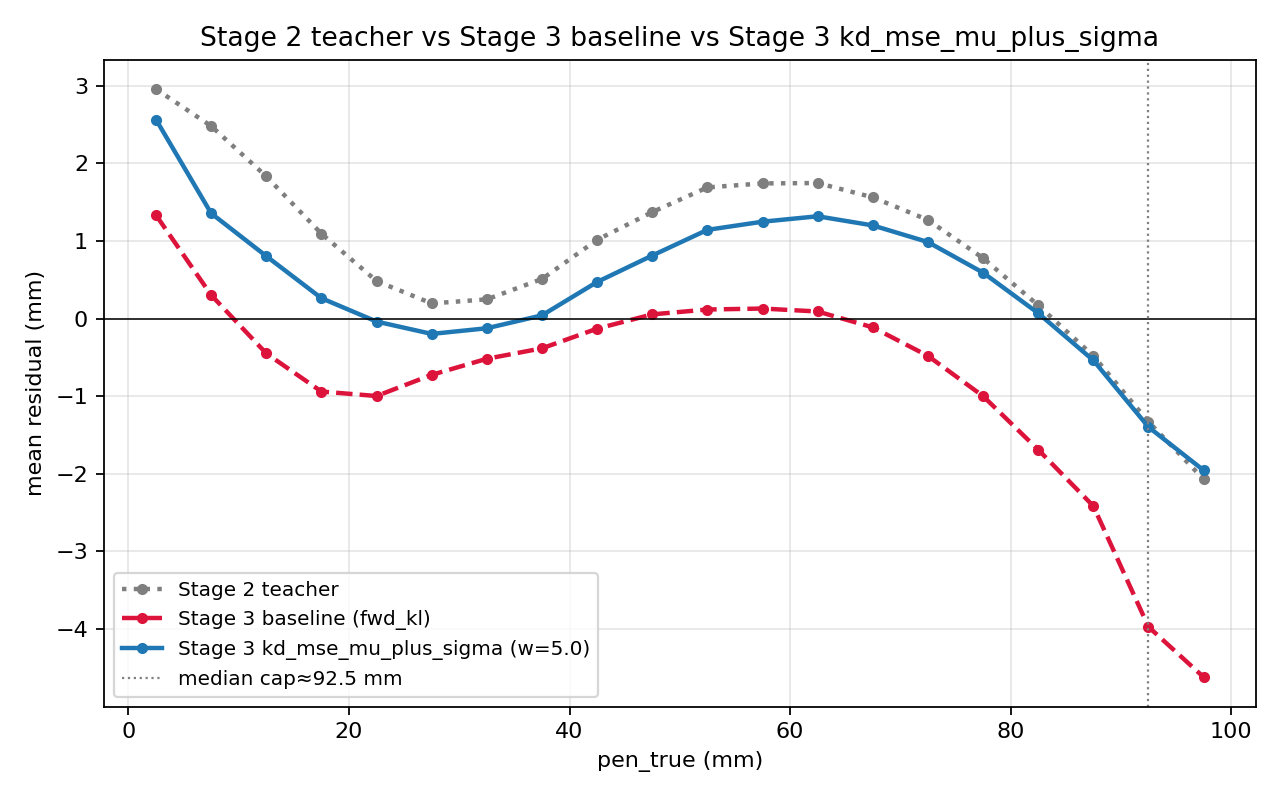
\includegraphics[width=\linewidth]{images/neural_network_fit_results/stage3_kd_mse_mu_plus_sigma_overlay_baseline.png}
\caption{Bias--truth curves.}
\end{subfigure}
\hfill
\begin{subfigure}[t]{0.49\linewidth}
\centering
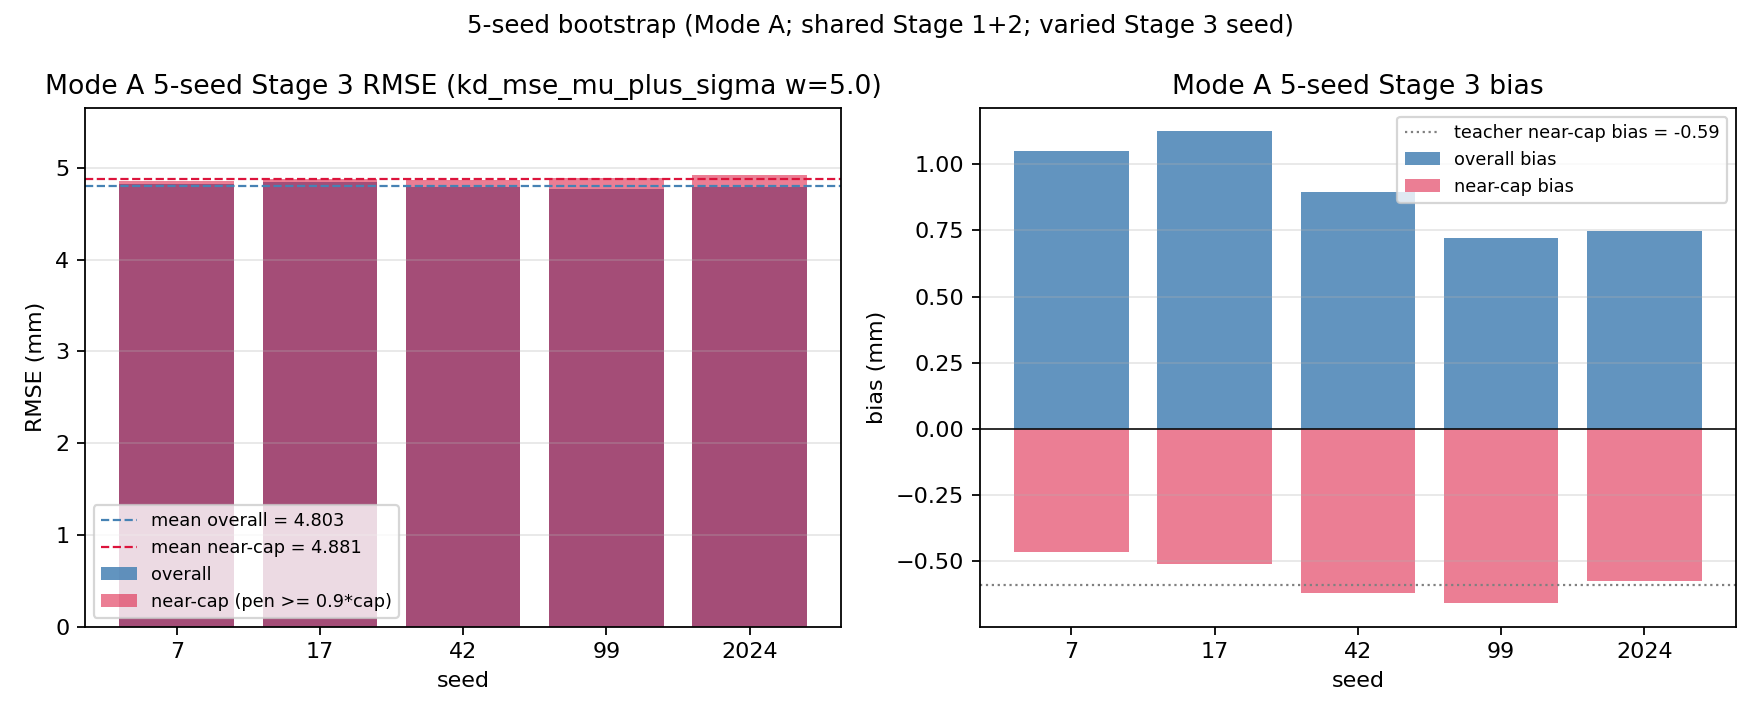
\includegraphics[width=\linewidth]{images/neural_network_fit_results/stage3_kd_mse_mu_plus_sigma_modeA_per_seed.png}
\caption{Five-seed stability.}
\end{subfigure}
\caption{Archived KD-form diagnostics. The mixed distillation loss repairs the near-cap bias while preserving stable five-seed behavior.}
\label{fig:kd-form-rewrite}
\end{figure}

\subsubsection{Post-Hoc Adaptation: Residual, FiLM, and SVGP Extensions}
\label{sec:posthoc-residual-rewrite}

The residual-adaptation analysis is useful, but it must be kept in the correct
evidential tier. It is a post-hoc extension, not the deployed-surrogate verdict.
In the staged-learning language introduced earlier, the Stage~1--3 MLP is the
base screening surrogate, while the residual-head and FiLM variants test
lightweight post-training adaptation around that base predictor. The SVGP
residual variants test the same adaptation idea with a sharper kernel
backbone.

The residual multi-task SVGP is an additive routed-residual model. In scaled
penetration space its mean has the form
\(\hat{y}(x,f)=g_{\mathrm{shared}}(x)+\Delta g_f(x)\), where
\(g_{\mathrm{shared}}\) is a frozen shared Stage~3 SVGP and \(\Delta g_f\) is a
zero-mean residual SVGP trained only for injector family \(f\). The family
identifier is deliberately not part of the kernel input vector; it only routes
each sample to the corresponding residual process. If a future family has no
trained residual process, the prediction falls back to the shared SVGP with
\(\Delta g_f=0\). The implementation also trains a final shared log-variance GP
on the residual errors, so the mean correction and uncertainty model remain
separate.

In the refreshed fixed-table artifacts, the residual-SVGP family is the
strongest in-domain direction: the QC-retrained residual-SVGP reaches
\SI{3.848}{mm} RMSE on the primary QC-gated uncensored CDF table. The residual
MLP variants also clarify the role of injector conditioning, but they do not
replace the LONO conclusion because the residual-SVGP was not LONO-tested in
the same way as the main Stage~3 MLP and SVGP comparison. The refreshed
design-comparison and climb tables, together with the archived
adaptation-study figures, are collected in
Appendix~\ref{app:evaluation-diagnostics}.

\begin{table}[t]
\centering
\scriptsize
\setlength{\tabcolsep}{4pt}
\begin{tabularx}{\linewidth}{@{}L{0.29\linewidth}rrrY@{}}
\toprule
Adaptation or alternative arm & \(\Delta\)RMSE & \(\Delta\)MAE & 1$\sigma$ & Boundary \\
\midrule
Single-output thesis SVGP & -0.098 & -0.121 & 0.717 & Main alternative backbone; improves point error but not conservative coverage. \\
Residual-family-head MLP & +0.334 & +0.169 & 0.858 & Injector-conditioning fallback; does not improve the primary fixed-table error. \\
Residual-FiLM MLP & +0.216 & +0.057 & 0.798 & More flexible MLP adapter, but still behind the production mean on point error. \\
Residual-SVGP & -0.264 & -0.178 & 0.761 & Strong in-domain follow-up; transfer remains untested under matching LONO. \\
QC-retrained residual-SVGP & \textbf{-0.337} & \textbf{-0.227} & 0.773 & Best fixed-table point result; transfer still needs matching LONO. \\
\bottomrule
\end{tabularx}
\caption{Incremental post-hoc adaptation evidence on the refreshed primary fixed table. Deltas are relative to the five-seed production MLP mean, so negative values improve RMSE or MAE; the \(1\sigma\) column shows that the lower-error arms are generally less conservative than the production MLP. The table is interpreted as a future-development signal, not as a replacement for the deployed-surrogate verdict.}
\label{tab:posthoc-residual-rewrite}
\end{table}

The residual-MLP LONO follow-up supports a narrower claim: inside the modified
injector family, the residual conversion repairs much of the bias of the
deployed nozzle head. Across the in-family folds, the residual head reduces
RMSE from about \SI{7.44}{mm} to about \SI{5.16}{mm}. This is evidence for
within-family adaptation, not proof of zero-shot generalization to a genuinely
new injector family.

The broader conclusion is that injector identity is useful as a conditioning
variable. It allows the surrogate to learn family-specific offsets and partly
repair nozzle-dependent bias within the supported design family. In this sense,
the residual-head and FiLM variants behave like lightweight post-training
adaptation around a shared base surrogate, and the residual multi-task SVGP
implements the same idea with routed family residual processes. However, this
should not be described as true zero-shot fine-tuning. The Nozzle0 and Nozzle6
stress cases show the boundary: an injector identifier or output residual can
shift a learned representation, but it cannot synthesize trunk-level features
for an unseen design family that the shared surrogate never represented.

\begin{figure}[t]
\centering
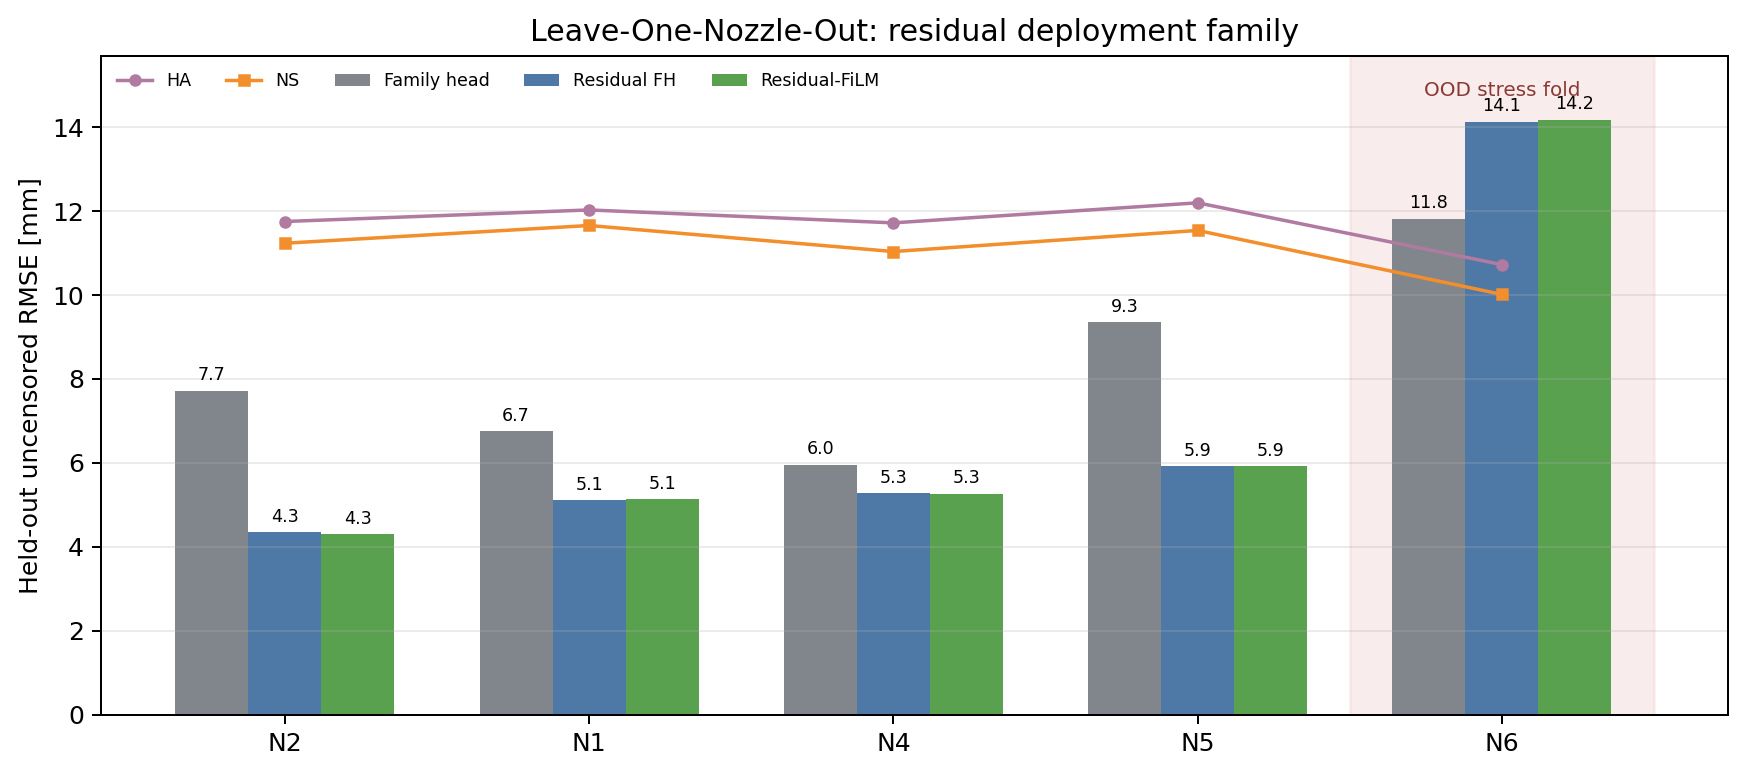
\includegraphics[width=0.86\linewidth]{images/residual_family_head_20260608/lono_modified_only_rmse_by_fold.png}
\caption{Archived residual-head LONO follow-up on modified-family nozzles. The residual adapter improves in-family folds but exposes its boundary on design-shifted cases.}
\label{fig:residual-lono-rewrite}
\end{figure}

\FloatBarrier

\subsection{Screening Demonstration and Evidence Boundary}
\label{sec:screening-boundary-rewrite}
\label{sec:prototype-screening-en}
\label{sec:prototype-screening-zh}

The final purpose of the surrogate is not just to minimize penetration error.
It is to feed a probabilistic geometric screening interface. The current GUI
prototype uses the MLP because the deployed MLP workflow also provides an
injection-onset auxiliary output for temporal screening displays. An SVGP could
replace the \(\mu,\sigma\) penetration channels, but it does not directly
provide this auxiliary onset output.

Under the default toy inputs used in the archived demonstration, the screening
prototype maps the predicted penetration distribution into a time-resolved
geometric interception score. For Design~A, the rank-oriented instantaneous
piston score peaks at \(P_{\mathrm{hit}}=77.66\%\), and the trapezoidal
cumulative exposure reaches \(E=\SI{2.475}{ms}\) by \SI{5}{ms}. Changing only
the geometry and kinematics changes the verdict: a wider bowl at the same
\SI{250}{rpm} increases \(E\) to \SI{3.364}{ms}, while a faster Hermite-profile
piston at \SI{2250}{rpm} reduces the cumulative exposure to
\SI{1.446}{ms} despite a high instantaneous opening.

\begin{figure}[t]
\centering
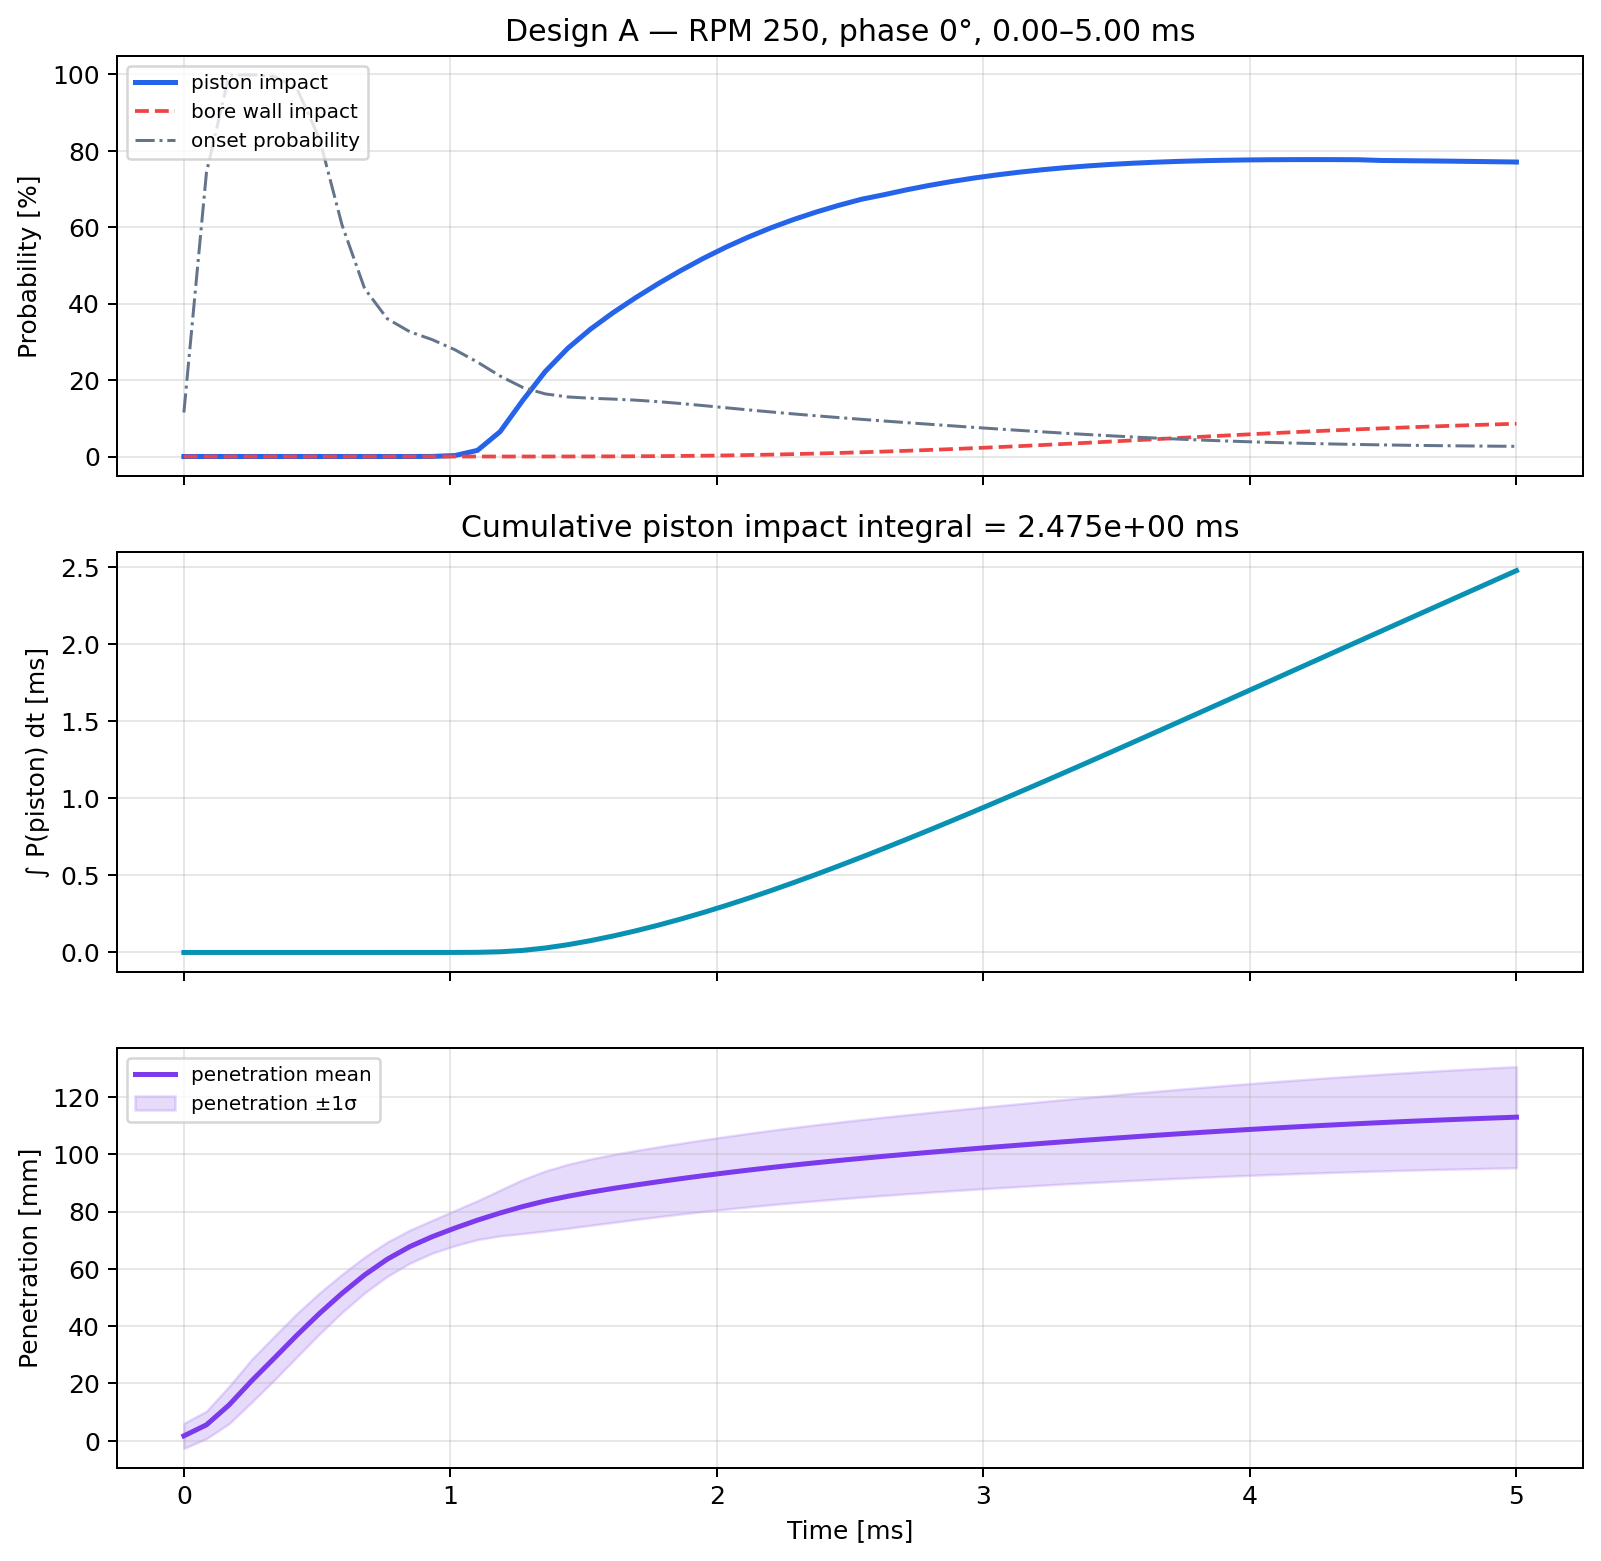
\includegraphics[width=0.82\linewidth]{images/impingement_summary.png}
\caption{Archived temporal summary of the wall-proximity screening prototype for Design~A. The output is a geometric screening score driven by the penetration distribution, not a measured liquid-wall-wetting probability.}
\label{fig:screening-design-a-rewrite}
\end{figure}

\begin{figure}[t]
\centering
\begin{subfigure}[t]{0.49\linewidth}
\centering
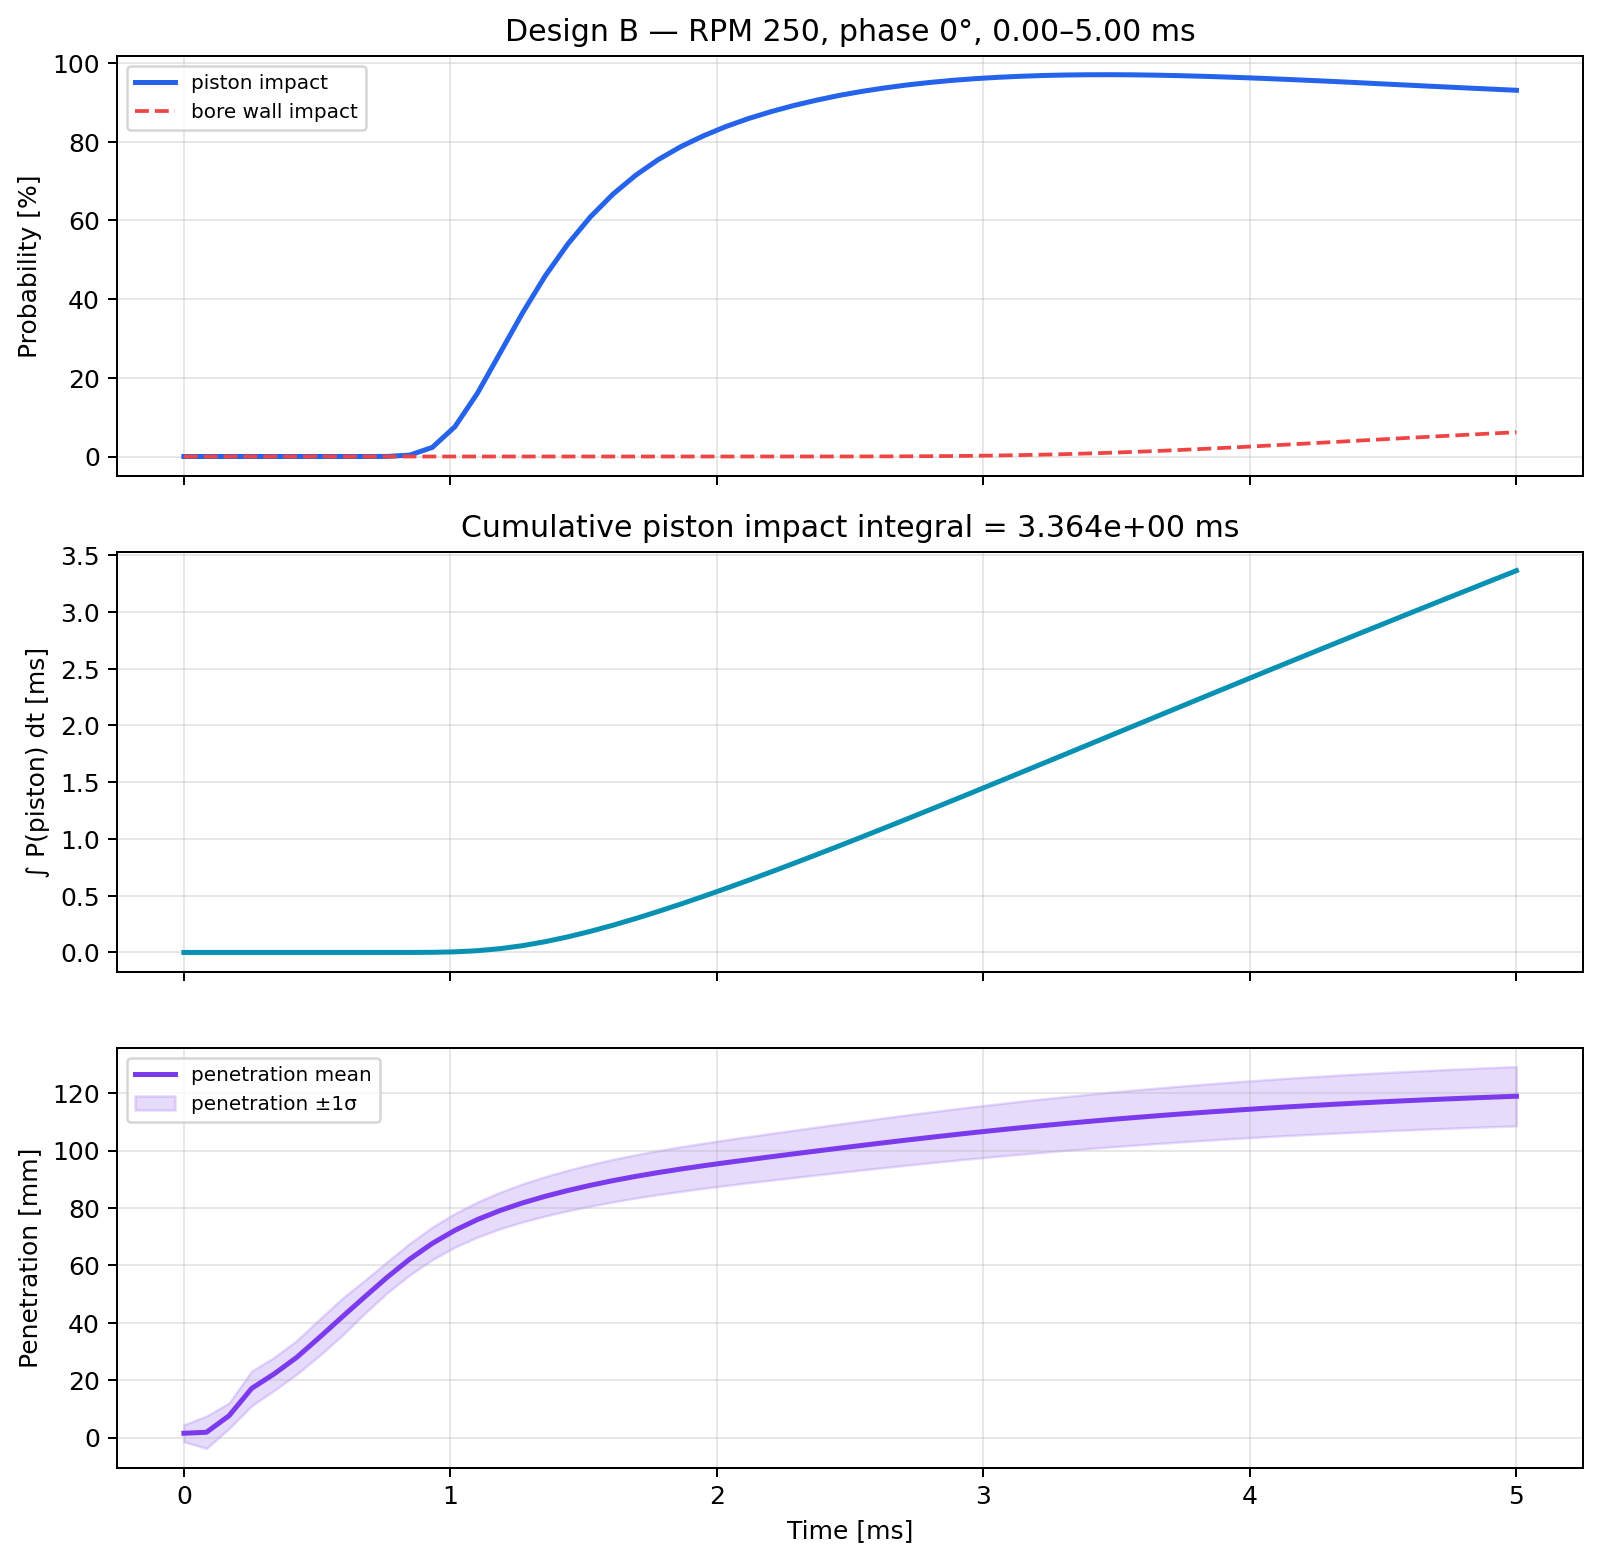
\includegraphics[width=\linewidth]{images/impingement_summary_design_b.png}
\caption{Design~B, wider bowl.}
\end{subfigure}
\hfill
\begin{subfigure}[t]{0.49\linewidth}
\centering
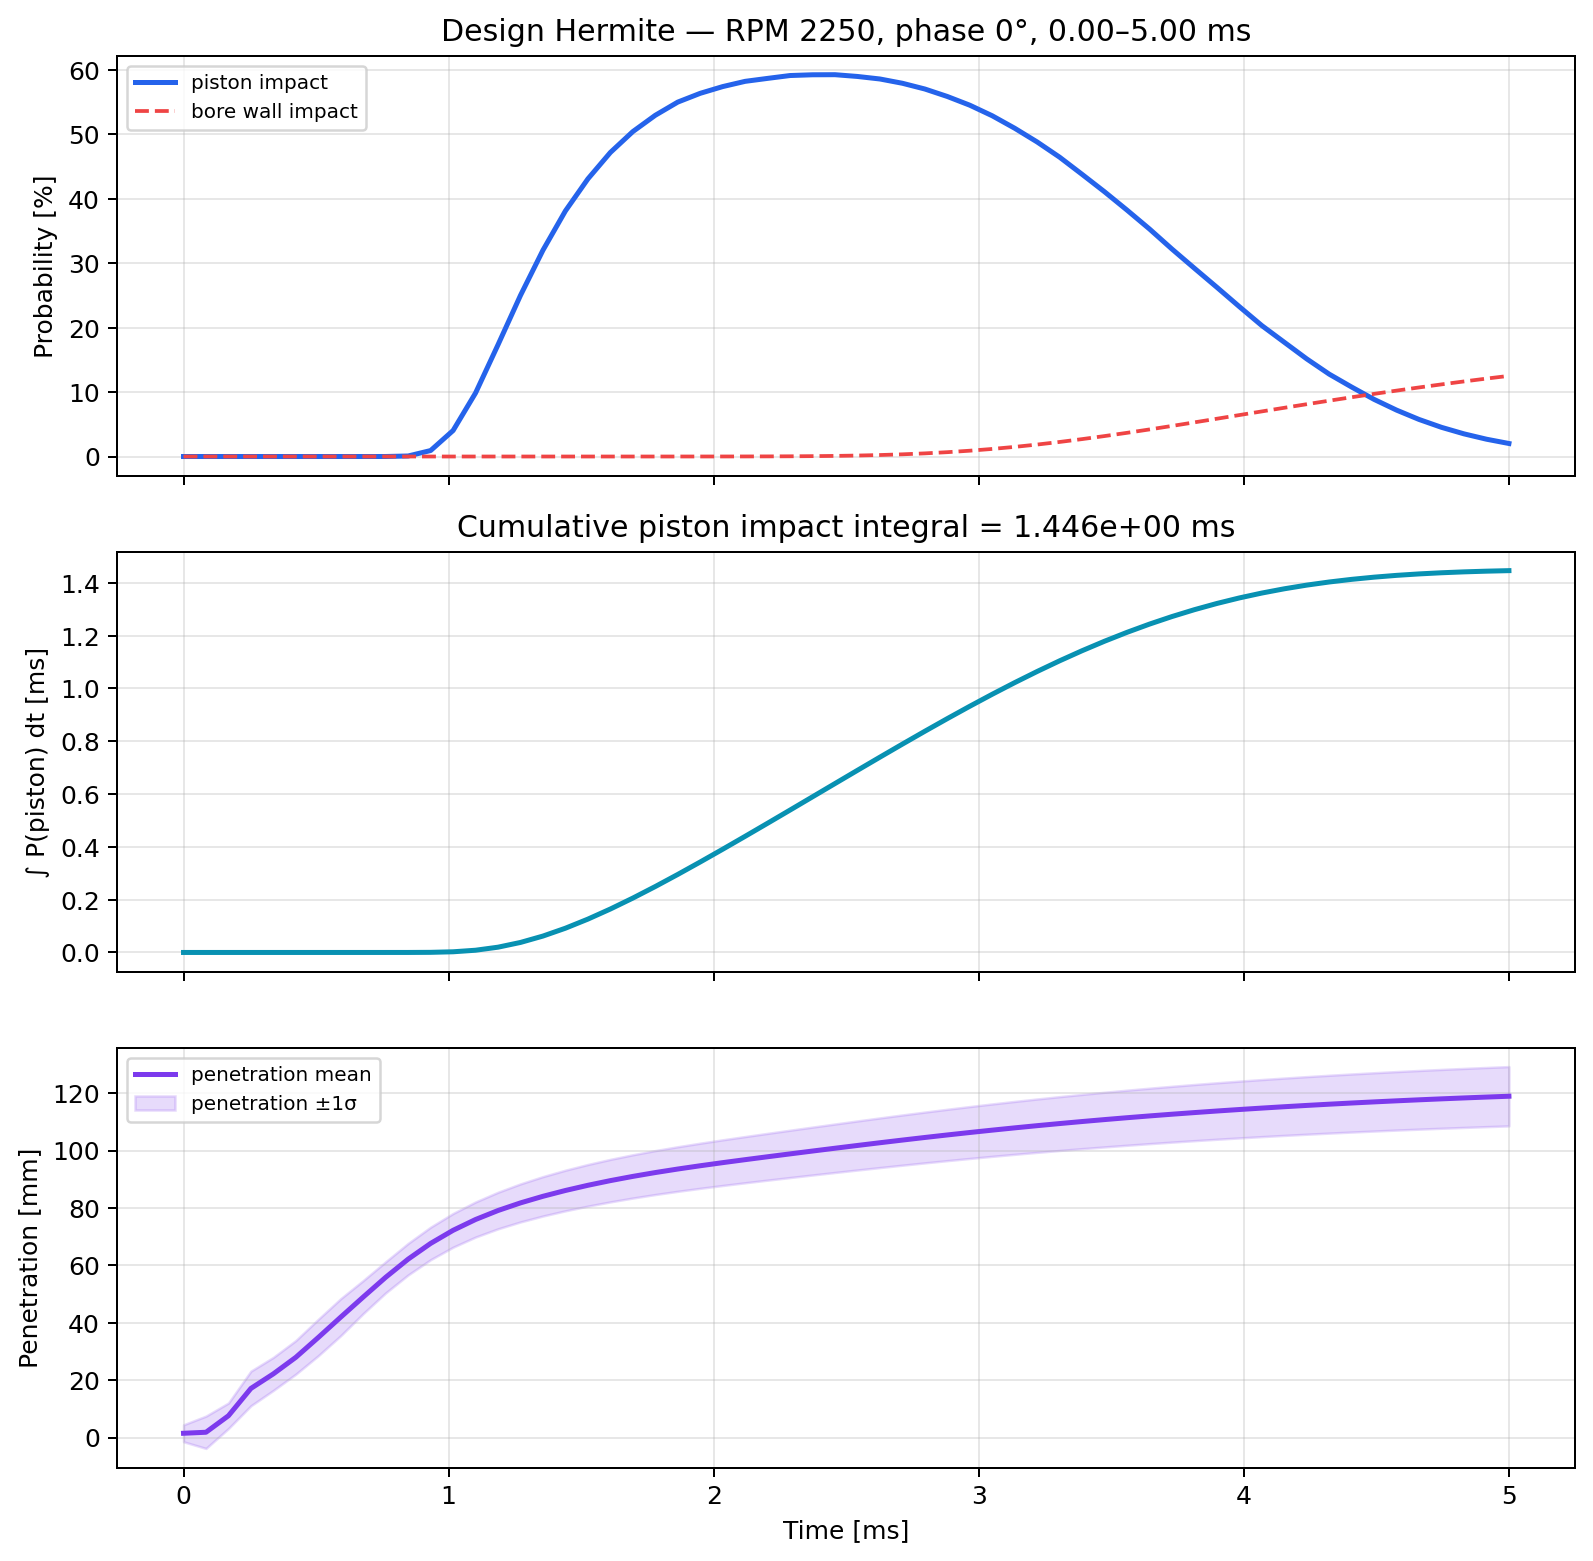
\includegraphics[width=\linewidth]{images/impingement_summary_design_hermite.png}
\caption{Hermite-profile piston.}
\end{subfigure}
\caption{Archived geometry and kinematics sensitivity of the screening layer. The same spray-side prediction can produce different rank-oriented screening scores after projection onto different piston motion profiles.}
\label{fig:screening-design-comparison-rewrite}
\end{figure}

The evidence boundary is essential. These interception scores are not
validated probabilities of harmful liquid-state impingement in an operating
engine. They are rank-oriented geometric screening metrics. The validated
contribution is the censoring-aware penetration surrogate over its measured
domain, together with a reproducible coupling from a predictive distribution to
a simplified screening interface.

\FloatBarrier

\subsection{Chapter Summary}
\label{sec:results-summary-rewrite}

Table~\ref{tab:chapter-verdict-rewrite} summarizes the chapter without
collapsing all protocols into a single ranking. Within the mainline deployed
comparison, the single-output SVGP is the better point predictor and the
production MLP is the more conservative screening surrogate. LONO transfer also
favors the SVGP for point accuracy and exposes Nozzle0 as a cross-design-family
failure for both architectures. The raw-image failure check shows why some
within-family plume trajectories remain difficult for smooth continuation
targets. Residual adaptation is promising, but it remains a post-hoc extension.
The screening demonstration closes the workflow while keeping the wall-impact
claim at the correct evidential level. Detailed per-fold, per-regime, and
residual-adaptation diagnostics, together with the archived claims-to-evidence
map of the earlier chapter organization, are collected in
Appendix~\ref{app:evaluation-diagnostics}.

\begin{table}[t]
\centering
\scriptsize
\setlength{\tabcolsep}{4pt}
\begin{tabularx}{\linewidth}{@{}L{0.22\linewidth}L{0.30\linewidth}Y@{}}
\toprule
Claim area & Best-supported result & Boundary \\
\midrule
In-domain fixed-table accuracy & Single-output thesis SVGP leads the mainline comparison at \SI{4.087}{mm} RMSE; production MLP mean is \SI{4.185}{mm}. & Residual arms are post-hoc adaptation evidence, not the deployed-surrogate verdict. \\
Conservative uncertainty & Production MLP has \(1\sigma/2\sigma\) coverage of 0.888/0.990, above the sharper SVGP variants. & Conservative coverage is useful for screening but is not a certified safety guarantee. \\
Condition-level behavior & Single-output thesis SVGP leads mainline P50 and q1 point error; q1 remains a hard positive-bias stress test. & q1 grid lacks CRPS/NLL in the refreshed artifacts, and post-hoc arms are interpreted separately. \\
Nozzle transfer & Archived LONO favors SVGP point transfer; excluding Nozzle0 gives SVGP \SI{5.95}{mm} vs. MLP \SI{7.00}{mm}. & Nozzle0 is a cross-design-family failure, not an ordinary fold. \\
Physical failure anatomy & Nozzle~3 images and curves show a flat-top, step-like transient trajectory that violates smooth continuation assumptions. & The images support a modeling failure-mode interpretation, not a unique causal fluid-mechanical diagnosis. \\
MLP workflow rationale & MLP is retained for conservative deployment, onset output, and affordable ablations. & This is a workflow argument, not a claim of universal predictive superiority. \\
Post-hoc adaptation & QC-retrained residual-SVGP is the in-domain frontier at \SI{3.848}{mm} RMSE; MLP residual adapters repair in-family bias. & Residual-SVGP transfer remains unverified under matching LONO. \\
Screening demo & Penetration distributions can be projected into geometry-sensitive rank scores. & Scores are geometric proxies, not validated liquid-impingement probabilities. \\
\bottomrule
\end{tabularx}
\caption{Condensed Results verdict. Each row states what the evidence supports and the boundary that prevents overclaiming.}
\label{tab:chapter-verdict-rewrite}
\end{table}

The next discussion chapter should therefore not re-run every metric. Its task
is to interpret the trade-off: the thesis establishes a reproducible
censoring-aware surrogate workflow with conservative uncertainty and a working
screening projection, while also showing that matching LONO tests for
residual-SVGP, larger post-training adaptation experiments, and controlled
last-block unfreezing are the likely next steps for point-accuracy
improvements.
